% ═══════════════════════════════════════════════════════════════════════
%  Apogée Invest — Guide pédagogique client (FxMultiSleeve)
%  Réutilise le préambule editorial du rapport principal.
% ═══════════════════════════════════════════════════════════════════════
\documentclass[11pt, a4paper]{scrartcl}

% ═══════════════════════════════════════════════════════════════════════
%  Phase 18 — Rapport de stratégie FX
%  Préambule LaTeX (XeLaTeX + KOMA-Script)
% ═══════════════════════════════════════════════════════════════════════

% ── Language & fonts ──────────────────────────────────────────────
\usepackage{fontspec}
\usepackage{polyglossia}
\setdefaultlanguage{french}
\setotherlanguage{english}

\setmainfont{Latin Modern Roman}[
  Ligatures=TeX,
  Numbers={Proportional,OldStyle}
]
\setsansfont{Inter}[
  Scale=MatchLowercase,
  Extension=.otf,
  Path=/usr/share/fonts/opentype/inter/,
  UprightFont=Inter-Regular,
  BoldFont=Inter-Bold,
  ItalicFont=Inter-Italic,
  BoldItalicFont=Inter-BoldItalic
]
\setmonofont{Latin Modern Mono}[Scale=MatchLowercase]

% ── Geometry ──────────────────────────────────────────────────────
\usepackage[
  a4paper,
  top=2.5cm,
  bottom=2.8cm,
  left=2.6cm,
  right=2.6cm,
  headheight=14pt,
  footskip=1.2cm
]{geometry}

% ── Colors — editorial palette ────────────────────────────────────
\usepackage{xcolor}
\definecolor{primary}{HTML}{0B2545}   % deep navy
\definecolor{primaryLight}{HTML}{134074}
\definecolor{accent}{HTML}{CC6B2F}    % burnt orange
\definecolor{mrBlue}{HTML}{1F5582}
\definecolor{tsOrange}{HTML}{CC6B2F}
\definecolor{rsiGreen}{HTML}{2E8B57}
\definecolor{combinedBurgundy}{HTML}{8E1616}
\definecolor{slateGrey}{HTML}{4A4A4A}
\definecolor{lightGrey}{HTML}{E6E8EB}
\definecolor{softBlue}{HTML}{DAE6F0}
\definecolor{softRed}{HTML}{F9E2E2}
\definecolor{softYellow}{HTML}{FCF4D9}
\definecolor{softGreen}{HTML}{E3F2E6}

% ── Core packages ─────────────────────────────────────────────────
\usepackage{amsmath}
\usepackage{amssymb}
\usepackage{graphicx}
\graphicspath{{figures/}}
\usepackage{float}
\usepackage{booktabs}
\usepackage{longtable}
\usepackage{array}
\usepackage{tabularx}
\usepackage{multicol}
\usepackage{multirow}
\usepackage{caption}
\usepackage{subcaption}
\usepackage{csquotes}
\usepackage{enumitem}
\setlist{nosep, leftmargin=*, labelsep=0.5em}

% siunitx for aligned numerical columns
\usepackage{siunitx}
\sisetup{
  group-separator={\,},
  output-decimal-marker={,},
  detect-weight=true,
  detect-family=true
}

% Captions — compact editorial style
\captionsetup{
  font={small},
  labelfont={bf, color=primary},
  textfont={it},
  labelsep=period,
  format=plain,
  width=0.95\textwidth
}

% ── Section titles — coloured bar style ──────────────────────────
\usepackage{titlesec}
\titleformat{\section}
  {\sffamily\Large\bfseries\color{primary}}
  {\thesection}{0.8em}{}
  [\vspace{-0.3em}{\color{accent}\rule{\linewidth}{1.2pt}}]
\titleformat{\subsection}
  {\sffamily\large\bfseries\color{primaryLight}}
  {\thesubsection}{0.6em}{}
\titleformat{\subsubsection}
  {\sffamily\normalsize\bfseries\color{slateGrey}}
  {\thesubsubsection}{0.5em}{}

\titlespacing*{\section}{0pt}{1.8em}{0.9em}
\titlespacing*{\subsection}{0pt}{1.2em}{0.5em}
\titlespacing*{\subsubsection}{0pt}{0.9em}{0.3em}

% ── Page headers / footers ───────────────────────────────────────
\usepackage{fancyhdr}
\pagestyle{fancy}
\fancyhf{}
\fancyhead[L]{\footnotesize\color{slateGrey}\textsf{Stratégie FX Tri-Signaux}}
\fancyhead[R]{\footnotesize\color{slateGrey}\textsf{\leftmark}}
\fancyfoot[C]{\footnotesize\color{slateGrey}\thepage}
\fancyfoot[R]{\footnotesize\color{slateGrey}\textsf{Rapport d'investissement --- Avril 2026}}
\renewcommand{\headrulewidth}{0.4pt}
\renewcommand{\footrulewidth}{0.0pt}
\renewcommand{\headrule}{\color{primary}\hrule width\headwidth height\headrulewidth}

% Show only section name in the right header, no number
\renewcommand{\sectionmark}[1]{\markboth{#1}{}}

% ── Tcolorbox — callouts ─────────────────────────────────────────
\usepackage[most]{tcolorbox}

\newtcolorbox{insightbox}[1][]{
  enhanced,
  colback=softBlue,
  colframe=primary,
  boxrule=0.8pt,
  arc=2pt,
  left=10pt, right=10pt, top=8pt, bottom=8pt,
  title=\textbf{\color{white}\textsf{Idée clé}},
  coltitle=white,
  fonttitle=\bfseries,
  attach boxed title to top left={xshift=8pt, yshift=-8pt},
  boxed title style={
    colback=primary,
    colframe=primary,
    arc=2pt,
    boxrule=0pt,
    left=6pt, right=6pt, top=2pt, bottom=2pt
  },
  #1
}

\newtcolorbox{warningbox}[1][]{
  enhanced,
  colback=softRed,
  colframe=combinedBurgundy,
  boxrule=0.8pt,
  arc=2pt,
  left=10pt, right=10pt, top=8pt, bottom=8pt,
  title=\textbf{\color{white}\textsf{Avertissement}},
  coltitle=white,
  fonttitle=\bfseries,
  attach boxed title to top left={xshift=8pt, yshift=-8pt},
  boxed title style={
    colback=combinedBurgundy,
    colframe=combinedBurgundy,
    arc=2pt,
    boxrule=0pt,
    left=6pt, right=6pt, top=2pt, bottom=2pt
  },
  #1
}

\newtcolorbox{examplebox}[1][]{
  enhanced,
  colback=softYellow,
  colframe=accent,
  boxrule=0.7pt,
  arc=2pt,
  left=10pt, right=10pt, top=8pt, bottom=8pt,
  title=\textbf{\color{white}\textsf{Exemple concret}},
  coltitle=white,
  fonttitle=\bfseries,
  attach boxed title to top left={xshift=8pt, yshift=-8pt},
  boxed title style={
    colback=accent,
    colframe=accent,
    arc=2pt,
    boxrule=0pt,
    left=6pt, right=6pt, top=2pt, bottom=2pt
  },
  #1
}

\newtcolorbox{thesisbox}[1][]{
  enhanced,
  colback=softGreen,
  colframe=rsiGreen,
  boxrule=0.7pt,
  arc=2pt,
  left=10pt, right=10pt, top=8pt, bottom=8pt,
  title=\textbf{\color{white}\textsf{Thèse économique}},
  coltitle=white,
  fonttitle=\bfseries,
  attach boxed title to top left={xshift=8pt, yshift=-8pt},
  boxed title style={
    colback=rsiGreen,
    colframe=rsiGreen,
    arc=2pt,
    boxrule=0pt,
    left=6pt, right=6pt, top=2pt, bottom=2pt
  },
  #1
}

% ── Drop caps ────────────────────────────────────────────────────
\usepackage{lettrine}
\renewcommand{\LettrineFontHook}{\color{primary}\bfseries}

% ── Hyperref (load last) ─────────────────────────────────────────
\usepackage[
  colorlinks=true,
  linkcolor=primary,
  citecolor=primary,
  urlcolor=accent,
  pdfborder={0 0 0},
  bookmarks=true,
  bookmarksnumbered=true,
  pdftitle={Stratégie FX Tri-Signaux --- Rapport d'investissement},
  pdfauthor={Thomas Vaudescal},
  pdfsubject={Stratégie quantitative FX diversifiée à trois moteurs de rendement},
  pdfkeywords={FX, mean reversion, momentum, portfolio, risk management}
]{hyperref}

% ── Custom commands ──────────────────────────────────────────────
\newcommand{\code}[1]{\texttt{\small #1}}
\newcommand{\sleeve}[1]{\textbf{\color{primary}#1}}
\newcommand{\metric}[1]{\textbf{\color{accent}#1}}

% Line spacing
\linespread{1.08}


% \rowcolor vient de colortbl, que le préambule partagé ne charge pas : le
% document l'utilise depuis toujours, et les compilations antérieures passaient
% l'erreur sans s'arrêter faute de -halt-on-error.
\usepackage[table]{xcolor}

% Override paths/headers pour ce document
\graphicspath{{figures/}{../../docs/logo/}{../latex_report/figures/}}
\fancyfoot[R]{\footnotesize\color{slateGrey}\textsf{Guide pédagogique client --- Mai 2026}}
\fancyhead[L]{\footnotesize\color{slateGrey}\textsf{FxMultiSleeve --- Comprendre la stratégie}}

\hypersetup{
  pdftitle={Stratégie FX Multi-Moteurs --- Guide pédagogique client},
  pdfsubject={Comprendre la stratégie FxMultiSleeve : moteurs, paramètres, gestion du risque},
  pdfkeywords={FX, mean reversion, momentum, RSI, MetaTrader 5, pédagogie}
}

\begin{document}

% ═══════════════════════════════════════════════════════════════════════
%  PAGE 1 — COUVERTURE
% ═══════════════════════════════════════════════════════════════════════
\thispagestyle{empty}
\begin{center}

\vspace*{-1.5cm}
\noindent{\color{apogeeGold}\rule{\textwidth}{2pt}}

\vspace{1.0cm}


\includegraphics[width=3.6cm]{apogee_invest_logo}

\vspace{0.3cm}

{\interspaced\color{apogeeGold}\normalsize\bfseries APOGÉE INVEST\par}

\vspace{0.3cm}

{\color{apogeeGold}\rule{0.28\textwidth}{0.5pt}}

\vspace{1.2cm}

{\interspaced\color{slateGrey}\footnotesize GUIDE PÉDAGOGIQUE CLIENT \enskip\textbullet\enskip COMPRENDRE LA STRATÉGIE\par}

\vspace{0.7cm}

{\sffamily\color{primary}\huge\bfseries
Stratégie FX Multi-Moteurs\par}

\vspace{0.4cm}

{\sffamily\color{accent}\Large\itshape
Logique, paramètres et gestion du risque\par}

\end{center}

\vspace{0.9cm}

\noindent\begin{minipage}{\textwidth}
\centering
{\color{apogeeGold}\rule{0.45\textwidth}{0.4pt}}\\[0.5em]
\begin{tabular}{@{}rl@{}}
  \color{slateGrey}\sffamily Document & \textbf{Guide pédagogique de la stratégie} \\[0.18em]
  \color{slateGrey}\sffamily Public & \textbf{Client final --- Onboarding et compréhension} \\[0.18em]
  \color{slateGrey}\sffamily Date & \textbf{Mai 2026} \\[0.18em]
  \color{slateGrey}\sffamily Statut & \textbf{Pédagogie --- complément du guide d'installation} \\[0.18em]
  \color{slateGrey}\sffamily Version & \textbf{1.0} \\
\end{tabular}\\[0.7em]
{\color{apogeeGold}\rule{0.45\textwidth}{0.4pt}}
\end{minipage}

\vspace{0.8cm}

\begin{thesisbox}
\textbf{Objectif de ce guide.} Vous expliquer \emph{pourquoi} la stratégie
FxMultiSleeve fonctionne, \emph{comment} chacun de ses quatre moteurs prend ses
décisions, et \emph{quels paramètres} influencent quoi. Ce document n'est pas un
manuel d'installation~--- pour cela, voir le \emph{Guide d'installation client}.
Ici, l'objectif est la compréhension : à la fin de la lecture, vous saurez lire
un rapport de backtest, juger si une intervention manuelle est requise, et
défendre les choix de conception devant un investisseur ou une banque dépositaire.
\end{thesisbox}

\vspace{0.4cm}

{\small\color{slateGrey}\sffamily
Ce guide complète : (i)~le \emph{guide d'installation} qui détaille la procédure
opérationnelle, (ii)~le \emph{rapport exécutif} qui synthétise les performances
en 10~pages pour un comité d'investissement, et (iii)~le \emph{rapport
quantitatif complet} qui documente la méthodologie de validation. Le présent
document se concentre sur la pédagogie de la stratégie elle-même : intuition
économique, mécanique des signaux, signification de chaque paramètre.}

\vfill

\noindent\colorbox{lightGrey}{%
  \makebox[\textwidth][l]{%
    \parbox{0.95\textwidth}{%
      \vspace{0.3cm}
      \footnotesize\color{slateGrey}\sffamily
      \textbf{Confidentiel.} Document destiné au client final d'Apogée~Invest.
      Performances issues de \emph{backtests} historiques. Les performances passées
      ne préjugent pas des performances futures. Toute décision d'investissement
      doit prendre en compte le risque de perte en capital.
      \vspace{0.3cm}
    }%
  }%
}

\newpage

% ═══════════════════════════════════════════════════════════════════════
%  TABLE DES MATIÈRES
% ═══════════════════════════════════════════════════════════════════════
{\hypersetup{linkcolor=primary}
\renewcommand{\contentsname}{\sffamily\Large\bfseries\color{primary}Table des matières}
\tableofcontents}

\newpage

% ═══════════════════════════════════════════════════════════════════════
%  § 1 — VUE D'ENSEMBLE
% ═══════════════════════════════════════════════════════════════════════
\section{Vue d'ensemble}
\label{sec:overview}

\lettrine[lines=2, findent=2pt, nindent=0pt]{F}{x}MultiSleeve est une stratégie quantitative diversifiée sur le marché des changes (FX) déployée en un seul \emph{Expert Advisor} sur MetaTrader~5. Elle combine \textbf{quatre moteurs de rendement indépendants}~--- trois sur les devises, un sur l'or~--- chacun spécialisé dans un régime de marché différent, regroupés sous une couche commune de gestion du risque.

\subsection{Le mandat client}

Le contrat avec Apogée Invest impose trois contraintes de premier ordre que la stratégie respecte sur sa fenêtre de validation 2020--2026~:

\begin{itemize}
\item \textbf{Rendement annualisé (CAGR)} dans l'intervalle $[10\,\%,\,15\,\%]$~;
\item \textbf{Aucun plafond de repli}~: le mandant a retiré cette contrainte~;
\item \textbf{Philosophie risk-first}~: la priorité est la \emph{robustesse hors échantillon} plutôt que la maximisation du Sharpe in-sample, ce qui implique une discipline forte de validation statistique et de \emph{guardrails} de risque.
\end{itemize}

\begin{insightbox}
\textbf{Pourquoi quatre moteurs plutôt qu'un seul ?} Parce que chaque régime de
marché favorise des inefficiences différentes. Un moteur unique~--- aussi bon
soit-il~--- subit des périodes prolongées de drawdown lorsque son régime favori
disparaît. La combinaison de trois signaux \emph{décorrélés} (intraday vs daily,
mean reversion vs momentum) lisse la courbe d'équité et réduit la sévérité des
phases de creux. C'est le principe de la diversification temporelle et stylistique.
\end{insightbox}

\subsection{Quatre moteurs, une seule philosophie}

Les trois moteurs FX partagent une racine commune : ils exploitent tous des \emph{anomalies micro-structurelles} bien documentées dans la littérature académique sur le marché des changes, plutôt que de s'appuyer sur des prédictions macroéconomiques discrétionnaires. Le quatrième, sur l'or, relève de la même discipline mais d'une littérature différente~--- le \emph{time series momentum}. Cette discipline rend le système \emph{auditable} et \emph{testable}, et limite la dérive comportementale.

\begin{itemize}
\item Le \sleeve{Moteur~1 (MR Macro)} capture la \emph{mean reversion} intraday autour du VWAP en horaires de forte liquidité, filtré par un régime macroéconomique sain.
\item Le \sleeve{Moteur~2 (TS Momentum)} capture les tendances FX lentes induites par les divergences de politique monétaire entre banques centrales, sur un horizon journalier.
\item Le \sleeve{Moteur~3 (RSI Daily)} capture les \emph{overshoot} statistiques de court terme via le RSI, en s'activant exactement quand les deux autres moteurs sont en creux.
\item Le \sleeve{Moteur~4 (Gold Momentum)} capture le \emph{time series momentum} de l'or sur des horizons de plusieurs semaines. C'est le seul moteur hors devises, et la source de rendement dominante du portefeuille (cf.~\ref{sec:gold}).
\end{itemize}

\subsection{Allocation et levier}

Le portefeuille combine les quatre moteurs avec une allocation statique et une couche commune de ciblage de volatilité~:

\begin{center}
\renewcommand{\arraystretch}{1.2}
\begin{tabular}{lcccc}
\toprule
\textbf{Moteur} & \textbf{Allocation} & \textbf{Timeframe} & \textbf{Style} & \textbf{Univers} \\
\midrule
\rowcolor{softBlue} Moteur 1 --- MR Macro & $72\,\%$ & M1 intraday & Mean reversion & 4 majors \\
\rowcolor{softYellow} Moteur 2 --- TS Momentum & $10\,\%$ & D1 swing & Trend following & 3 majors \\
\rowcolor{softGreen} Moteur 3 --- RSI Daily & $10\,\%$ & D1 swing & Mean reversion & 3 majors \\
\bottomrule
\end{tabular}
\end{center}

Au-dessus de cette allocation, un \textbf{ciblage de volatilité global} ajuste quotidiennement le levier appliqué de façon à maintenir une volatilité réalisée du portefeuille proche de $37\,\%$ annualisé (cible élevée, justifiée par la diversification entre moteurs). Le levier est plafonné à $31\times$ et est recalculé chaque jour à 21h~UTC sur la base de la volatilité observée des 21 et 63 derniers jours.

\begin{warningbox}
\textbf{Les chiffres de levier (jusqu'à $31\times$) supposent un compte bancaire
US offshore ou un compte EU \enquote{Professionnel} avec capital significatif.}
Sur un compte EU retail standard plafonné à $30\times$ par les règles ESMA, la
stratégie reste opérationnelle mais le \emph{return on equity} est mécaniquement
réduit. Le sizing s'adapte automatiquement au levier maximum disponible.
\end{warningbox}

\newpage

% ═══════════════════════════════════════════════════════════════════════
%  § 2 — ARCHITECTURE
% ═══════════════════════════════════════════════════════════════════════
\section{Architecture des quatre moteurs}
\label{sec:architecture}

\subsection{Vue synthétique}

Chaque moteur est une stratégie autonome avec son propre univers de paires, ses propres indicateurs, et ses propres règles d'entrée et de sortie. Ils se partagent uniquement~:

\begin{itemize}
\item Le \emph{sub-equity} virtuel calculé par la couche de risque (allocation $\times$ equity totale)~;
\item Le levier global recalculé chaque jour~;
\item Les disjoncteurs (DD-cap, margin-cap) qui peuvent forcer une fermeture coordonnée.
\end{itemize}

\subsection{Tableau comparatif}

\begin{center}
\renewcommand{\arraystretch}{1.3}
\small
\begin{tabular}{p{3.2cm}p{3.5cm}p{3.5cm}p{3.5cm}}
\toprule
 & \cellcolor{softBlue}\textbf{Moteur 1} & \cellcolor{softYellow}\textbf{Moteur 2} & \cellcolor{softGreen}\textbf{Moteur 3} \\
 & \cellcolor{softBlue}MR Macro & \cellcolor{softYellow}TS Momentum & \cellcolor{softGreen}RSI Daily \\
\midrule
Allocation & 72\,\% & 9\,\% & 9\,\% \\
Timeframe & M1 (1 minute) & D1 (1 jour) & D1 (1 jour) \\
Type & Mean reversion intraday & Suivi de tendance & Mean reversion swing \\
Indicateurs & VWAP + Bollinger 5\,$\sigma$ & EMA 20/50 + RSI(7) & RSI(14) \\
Univers & EUR/USD, GBP/USD, USD/JPY, USD/CAD & EUR/USD, GBP/USD, USD/JPY & EUR/USD, GBP/USD, USD/CAD \\
Filtres & Session 8-16 UTC, macro, news USD & --- & --- \\
Sortie & Stop, take-profit, time-stop 6h, EOD 21h & Inversion du signal & Retour RSI vers 50, time-stop 21j \\
Trades / an & $\sim 60$ & $\sim 90$ & $\sim 7$ \\
Win rate & $\sim 58\,\%$ & $\sim 64\,\%$ & $\sim 71\,\%$ \\
Rôle dans le P\&L & \emph{Workhorse} ($\sim 56\,\%$) & Marginal ($\sim 8\,\%$) & Diversificateur ($\sim 39\,\%$) \\
\bottomrule
\end{tabular}
\end{center}

\subsection{Pourquoi cette répartition de poids ?}

\begin{thesisbox}
\textbf{Le poids reflète le rapport rendement/volatilité, pas la part du P\&L.}
Le Moteur~1 reçoit 72\,\% parce qu'il a la volatilité intrinsèque la plus basse
(environ $1.3\,\%$ annualisé) couplée au Sharpe le plus élevé. Lui allouer une
fraction importante du capital ne le rend pas plus risqué que les autres
moteurs~--- au contraire, en termes de \emph{contribution au risque}, les trois
moteurs FX sont approximativement équipondérés.

\smallskip
Le Moteur~4 échappe à cette logique~: ses $10\,\%$ ne sont pas un poids
vol-équipondéré mais un plafond d'exposition délibéré. Sa volatilité propre
($33.9\,\%$ annualisée) est d'un ordre de grandeur au-dessus de celle des moteurs
FX, si bien qu'à $10\,\%$ du capital il porte déjà l'essentiel du risque \emph{et}
du rendement du portefeuille. C'est un choix assumé, discuté en~\ref{sec:gold}.
\end{thesisbox}

Cette logique \emph{vol-équipondérée}, classique en construction de portefeuille institutionnel, s'oppose à une équipondération naïve $33/33/33$ qui aurait sur-pondéré les moteurs daily volatils au détriment du moteur intraday régulier.

\subsection{Performance combinée}

\begin{figure}[H]
\centering

\includegraphics[width=\linewidth]{equity_combined_logscale.png}
\caption{Courbe d'équité log-scale du portefeuille combiné FxMultiSleeve sur 2020--2026, avec décomposition par moteur. Les trois courbes ne se déplacent pas en synchrone~--- c'est précisément ce que permet la diversification.}
\end{figure}

\begin{insightbox}
\textbf{La courbe combinée est plus régulière que chacune des composantes prise
séparément.} Lorsque l'un des moteurs traverse un creux, les deux autres compensent
souvent. C'est le profil que recherche un comité d'investissement~: un Sharpe
élevé n'a de valeur que s'il est stable dans le temps. Une stratégie unique à
Sharpe $1.5$ avec drawdowns de $30\,\%$ tous les 2~ans est moins attrayante qu'une
combinaison à Sharpe $1.3$ avec drawdowns plafonnés à $10\,\%$.
\end{insightbox}

\newpage

% ═══════════════════════════════════════════════════════════════════════
%  § 3 — MOTEUR 1 : MR MACRO
% ═══════════════════════════════════════════════════════════════════════
\section{Moteur 1 --- MR Macro (mean reversion intraday filtrée)}
\label{sec:mr_macro}

\subsection{Intuition économique}

\begin{thesisbox}
\textbf{La \emph{mean reversion} intraday fonctionne dans les régimes de
liquidité normale et de transmission monétaire saine.} Lorsque la courbe des
taux s'inverse ou que le taux de chômage commence à remonter, les
micro-structures qui rendent la \emph{mean reversion} profitable disparaissent~:
les flux deviennent unidirectionnels en raison de la \enquote{fuite vers la qualité},
les spreads s'élargissent, et toute prise de position à contre-courant devient
coûteuse. Le filtre macro bloque précisément la stratégie dans ces régimes.
\end{thesisbox}

Le moteur exploite deux asymétries micro-structurelles bien documentées sur le marché FX~:

\begin{enumerate}
\item La tendance des prix intraday à revenir vers le \textbf{VWAP} au cours de la session de chevauchement Londres / New~York, pendant laquelle les teneurs de marché rebalancent leurs inventaires.
\item La \textbf{surréaction de court terme} aux annonces macroéconomiques~: les déviations supérieures à cinq écarts-types autour du VWAP capturent typiquement une réaction excessive à une publication ou à un flux institutionnel concentré.
\end{enumerate}

\subsection{Mécanique du signal}

Le moteur repose sur quatre étages de décision séquentiels~:

\paragraph{Étage 1 --- Construire la référence VWAP.}
À chaque minute, on accumule la somme \texttt{prix~$\times$~volume~tick} divisée par la somme des volumes depuis 00h00~UTC. Le \emph{Volume-Weighted Average Price} ainsi obtenu sert de \emph{point pivot} : c'est le prix moyen pondéré par l'activité depuis le début de la journée.

\paragraph{Étage 2 --- Mesurer la déviation.}
On calcule \texttt{close~--~VWAP} pour chaque bougie M1 fermée, ce qui donne une série temporelle stationnaire sur laquelle on peut appliquer une statistique standard.

\paragraph{Étage 3 --- Bandes de Bollinger sur la déviation.}
On calcule la moyenne mobile et l'écart-type sur les 80 dernières observations de cette déviation. Les bandes inférieure et supérieure sont placées à $\pm 5\,\sigma$. Un signal d'achat se déclenche lorsque la déviation passe sous la bande inférieure (le prix est anormalement bas par rapport à sa propre dynamique de la journée), et symétriquement pour la vente.

\paragraph{Étage 4 --- Filtres autorisant le trade.}
Trois filtres doivent simultanément valider l'entrée~:
\begin{itemize}
\item \textbf{Session UTC} : l'heure courante doit être dans la fenêtre $[8\text{h}, 16\text{h}[$ qui couvre la session Londres complète et le démarrage de New~York.
\item \textbf{Régime macro} : le \emph{spread} 10Y-2Y des Treasuries américaines doit être inférieur à $0{,}5$ \emph{et} le taux de chômage US ne doit pas être en hausse sur 3 mois glissants.
\item \textbf{Fenêtre de news} : l'instant courant ne doit pas être dans une fenêtre de $\pm 15$~minutes autour d'une publication économique \enquote{high impact} américaine (NFP, CPI, FOMC, etc.).
\end{itemize}

\paragraph{Sorties.}
Trois mécanismes peuvent fermer une position~: \texttt{take-profit} à $+0{,}6\,\%$, \texttt{stop-loss} à $-0{,}5\,\%$, \texttt{time-stop} après 6 heures de détention, et \texttt{forced close} obligatoire à 21h~UTC pour ne jamais détenir une position pendant la phase de basse liquidité asiatique.

\subsection{Anatomie d'un trade}

\begin{examplebox}
\textbf{Lecture concrète~:} sur la figure ci-dessus, le prix touche la bande
inférieure vers 09h~UTC (déviation extrême à la baisse). La session est ouverte,
le filtre macro est passant, aucune publication n'est imminente~: le moteur
ouvre un long. Le prix revient vers le VWAP au bout de quelques heures, le
\emph{take-profit} se déclenche, et la position est fermée avec un gain~--- avant
même que le \emph{time-stop} ou la fermeture à 21h~UTC n'aient à intervenir.
\end{examplebox}

\subsection{Paramètres expliqués}

\begin{center}
\renewcommand{\arraystretch}{1.3}
\small
\begin{tabular}{p{3.4cm}p{1.8cm}p{8.2cm}}
\toprule
\textbf{Paramètre} & \textbf{Valeur} & \textbf{Pourquoi cette valeur ?} \\
\midrule
\code{Inp\_MR\_BBWindow} & $80$ & Fenêtre de 80~minutes capture la dynamique d'une session liquide complète. Trop court ($<40$) génère des faux signaux par bruit~; trop long ($>120$) lisse les anomalies exploitables. \\
\code{Inp\_MR\_BBAlpha} & $5{,}0$ & Multiplicateur de l'écart-type pour la bande. $5\,\sigma$ est volontairement extrême~: on ne trade que les vraies surréactions, pas les fluctuations normales. À $2\,\sigma$ on aurait dix fois plus de trades pour un edge dilué. \\
\code{Inp\_MR\_SLStop} & $0{,}005$ & Stop-loss à $0{,}5\,\%$. Calé sur le drawdown moyen toléré pour un retour à la moyenne intraday~; un stop plus serré ($0{,}3\,\%$) est trop souvent atteint par bruit, plus large ($1\,\%$) coûte trop cher en cas d'erreur. \\
\code{Inp\_MR\_TPStop} & $0{,}006$ & Take-profit à $+0{,}6\,\%$. Légèrement supérieur au stop pour avoir un \emph{reward/risk} positif~--- le retour vers le VWAP est typiquement plus large que la déviation initiale. \\
\code{Inp\_MR\_SessionStart} & $8$ & Heure UTC de début de fenêtre de trading. Démarre avec le \emph{fixing} de Londres ; trop tôt ($<6$) capture la phase asiatique illiquide. \\
\code{Inp\_MR\_SessionEnd} & $16$ & Heure UTC de fin. Couvre l'overlap Londres / New~York ; trop tard ($>17$) entre dans la phase post-fixing américain où la liquidité retombe. \\
\code{Inp\_MR\_TimeStopHours} & $6$ & Durée maximale d'une position. Si la mean reversion ne se déclenche pas en 6~heures, le signal était probablement vicié~: on ferme. \\
\code{Inp\_MR\_ForcedCloseHr} & $21$ & Fermeture obligatoire à 21h~UTC. Évite tout overnight, où le spread peut s'élargir et où un \emph{gap} de week-end pourrait blesser la position. \\
\code{Inp\_MR\_SpreadThresh} & $0{,}5$ & Seuil du \emph{spread} 10Y-2Y au-dessous duquel on autorise le trading. Au-dessus, la courbe est trop plate ou inversée, signalant un stress cyclique~: le moteur se met en pause. \\
\code{Inp\_MR\_NewsFilter\-Enabled} & \texttt{true} & Active le blackout de $\pm 15$~min autour des publications USD high-impact. Sans ce filtre, les trades exécutés pendant un \emph{spike} de spread perdent souvent malgré un signal correct. \\
\bottomrule
\end{tabular}
\end{center}

\subsection{Performance historique}

\begin{figure}[H]
\centering
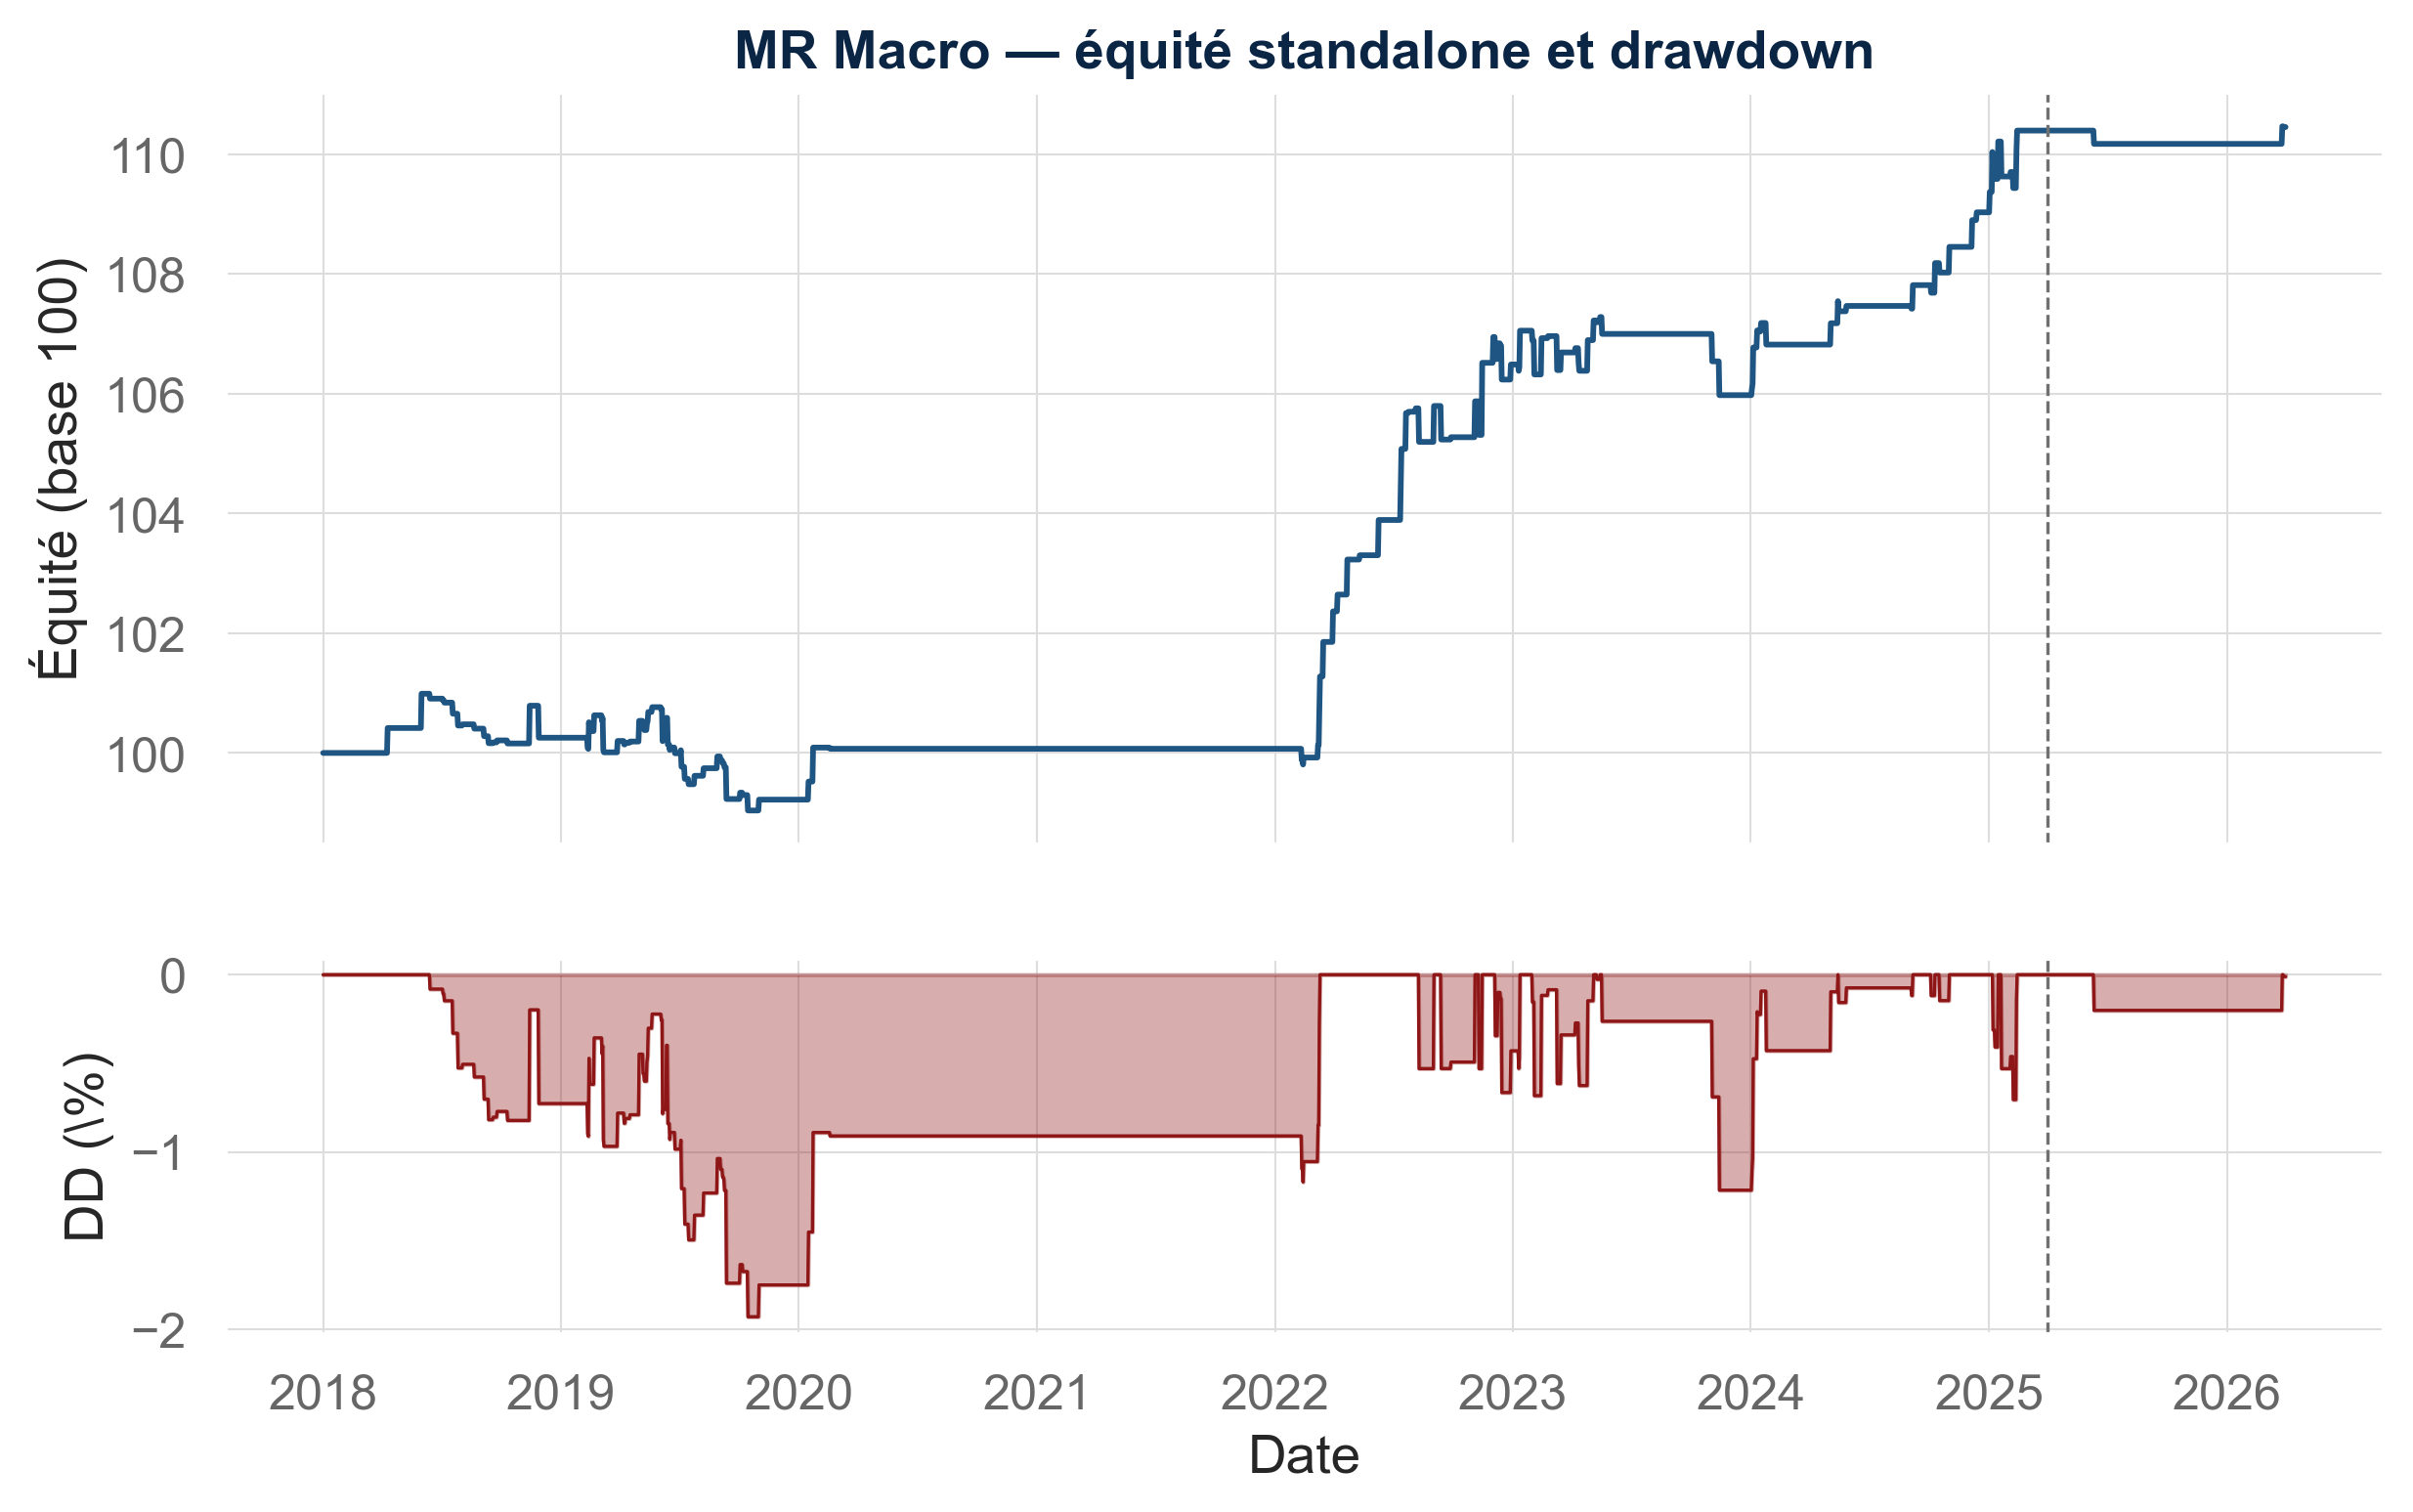
\includegraphics[width=\linewidth]{sleeve_mr_macro_equity.png}
\caption{Équité et drawdown du Moteur~1 pris isolément (non pondéré, non leveragé) sur 2019--2026. La ligne verticale pointillée marque le début de la fenêtre hors échantillon.}
\end{figure}

\begin{warningbox}
\textbf{Le filtre macro peut réduire la stratégie au silence complet pendant
plusieurs mois.} Sur 2021, aucun trade n'a été déclenché parce que la courbe
des taux est restée exceptionnellement raide après le choc Covid. Ce comportement
est \emph{voulu}~: la sensibilité des paramètres a démontré qu'assouplir le seuil
détruit la performance des autres années. Le \emph{silence sélectif} est une
propriété désirable du filtre, pas un bug.
\end{warningbox}

\newpage

% ═══════════════════════════════════════════════════════════════════════
%  § 4 — MOTEUR 2 : TS MOMENTUM
% ═══════════════════════════════════════════════════════════════════════
\section{Moteur 2 --- TS Momentum (suivi de tendance journalier)}
\label{sec:ts_momentum}

\subsection{Intuition économique}

\begin{thesisbox}
\textbf{Les divergences de politique monétaire entre grandes banques centrales
créent des tendances FX durables.} Lorsque la BCE et la Fed divergent~--- l'une
en cycle de hausse, l'autre en pause ou en baisse~--- le différentiel de taux
d'intérêt attendu se traduit par un mouvement directionnel du taux de change.
Ce mouvement est lent, déployé sur plusieurs semaines, et capturable par un
signal de tendance simple fondé sur un croisement de moyennes mobiles
exponentielles, combiné à une confirmation par l'indicateur RSI.
\end{thesisbox}

Trois mécanismes économiques sous-tendent ce signal~:

\begin{itemize}
\item \textbf{Forward guidance asymétrique} : lorsqu'une banque centrale télégraphie un cycle de hausse prolongé, le marché prend plusieurs semaines à intégrer l'ensemble de la trajectoire anticipée, créant une tendance lente exploitable.
\item \textbf{Carry roll-down} : le différentiel de taux courts induit un flux directionnel (\emph{carry trade}) qui renforce la tendance initiée.
\item \textbf{Rebalancement des réserves} : les banques centrales émergentes rebalancent leurs réserves USD/EUR/JPY en fonction des niveaux relatifs, créant des flux acheteurs ou vendeurs prévisibles à fréquence mensuelle.
\end{itemize}

\subsection{Mécanique du signal}

\begin{enumerate}
\item \textbf{EMA 20 et EMA 50} sur le close journalier de chaque paire. Le croisement (EMA20 au-dessus de EMA50 ou inversement) définit la direction.
\item \textbf{RSI(7)} comme filtre de confirmation pour éviter d'acheter au sommet ou vendre au creux~:
  \begin{itemize}
  \item Long si $\mathrm{EMA}_{\mathrm{fast}} > \mathrm{EMA}_{\mathrm{slow}}$ \emph{et} $\mathrm{RSI} < 60$.
  \item Short si $\mathrm{EMA}_{\mathrm{fast}} < \mathrm{EMA}_{\mathrm{slow}}$ \emph{et} $\mathrm{RSI} > 40$.
  \end{itemize}
\item \textbf{Lecture stricte sur barres fermées} : les indicateurs sont calculés sur \texttt{shift~=~1} (la veille), jamais sur la barre courante en formation. Cette discipline élimine tout risque de \emph{look-ahead bias}.
\item \textbf{Sizing par paire à volatilité ciblée} : le levier appliqué à chaque paire est $\min(0{,}10\,/\,\sigma_{21},\,3)$, où $\sigma_{21}$ est la volatilité réalisée sur 21~jours. Plus la paire est volatile, moins on engage de capital~--- le risque par trade reste constant.
\item \textbf{Sortie} : inversion du signal. Pas de stop dur autre qu'un filet de sécurité large à $-2\,\%$ pour gérer un \emph{gap} de week-end exceptionnel.
\end{enumerate}

\subsection{Pourquoi seulement trois paires ?}

L'univers initial à quatre paires (EUR/USD, GBP/USD, USD/JPY, USD/CAD) a été audité année par année. La paire USD/CAD est ressortie comme un mauvais contributeur récurrent~:

\begin{center}
\renewcommand{\arraystretch}{1.1}
\begin{tabular}{lrrrr}
\toprule
\textbf{Année} & \textbf{EUR-USD} & \textbf{GBP-USD} & \textbf{USD-JPY} & \textbf{USD-CAD} \\
\midrule
2019 & $-3{,}36\,\%$ & $+3{,}22\,\%$ & $+1{,}67\,\%$ & \textcolor{combinedBurgundy}{$-8{,}94\,\%$} \\
2022 & $+12{,}17\,\%$ & $+12{,}90\,\%$ & $+2{,}58\,\%$ & \textcolor{combinedBurgundy}{$-7{,}32\,\%$} \\
2023 & $-2{,}57\,\%$ & $+12{,}52\,\%$ & $+6{,}20\,\%$ & \textcolor{combinedBurgundy}{$-5{,}72\,\%$} \\
\bottomrule
\end{tabular}
\end{center}

L'explication économique~: USD/CAD est fortement \emph{range-bound} autour du prix du pétrole WTI et présente peu de tendances structurelles. Un signal de croisement EMA est inadapté à cette microstructure. Le retrait de USD/CAD de l'univers du Moteur~2 a augmenté son Sharpe de $0{,}44$ à $0{,}57$, soit un gain relatif de $30\,\%$.

\subsection{Paramètres expliqués}

\begin{center}
\renewcommand{\arraystretch}{1.3}
\small
\begin{tabular}{p{3.4cm}p{1.8cm}p{8.2cm}}
\toprule
\textbf{Paramètre} & \textbf{Valeur} & \textbf{Pourquoi cette valeur ?} \\
\midrule
\code{Inp\_TS\_FastEMA} & $20$ & Moyenne mobile rapide. $20$ jours $\approx$ un mois de trading, capture les tendances structurelles tout en filtrant le bruit hebdomadaire. \\
\code{Inp\_TS\_SlowEMA} & $50$ & Moyenne mobile lente. $50$ jours $\approx$ deux mois et demi, équivalent à un trimestre comptable~--- horizon naturel pour une révision de politique monétaire. \\
\code{Inp\_TS\_RSIPeriod} & $7$ & Période RSI courte. Réagit rapidement aux conditions de surachat / survente sans être trop bruyant. $14$ serait trop lent pour un filtre. \\
\code{Inp\_TS\_RSILow} & $40$ & Borne basse pour autoriser un short. Si le RSI est sous $40$, le marché est déjà fortement vendu~: on évite d'aggraver. \\
\code{Inp\_TS\_RSIHigh} & $60$ & Borne haute pour autoriser un long. Si le RSI est au-dessus de $60$, le marché est déjà fortement acheté~: on évite d'acheter au sommet. \\
\code{Inp\_TS\_TargetVol} & $0{,}10$ & Cible de volatilité par paire ($10\,\%$ annualisé). Calibre le sizing pour que chaque paire contribue le même risque, peu importe sa volatilité intrinsèque. \\
\code{Inp\_TS\_MaxLeverage} & $3{,}0$ & Plafond de levier individuel par paire. Empêche un sur-sizing en cas de paire anormalement calme (volatilité réalisée très basse). \\
\bottomrule
\end{tabular}
\end{center}

\subsection{Performance historique}

\begin{figure}[H]
\centering
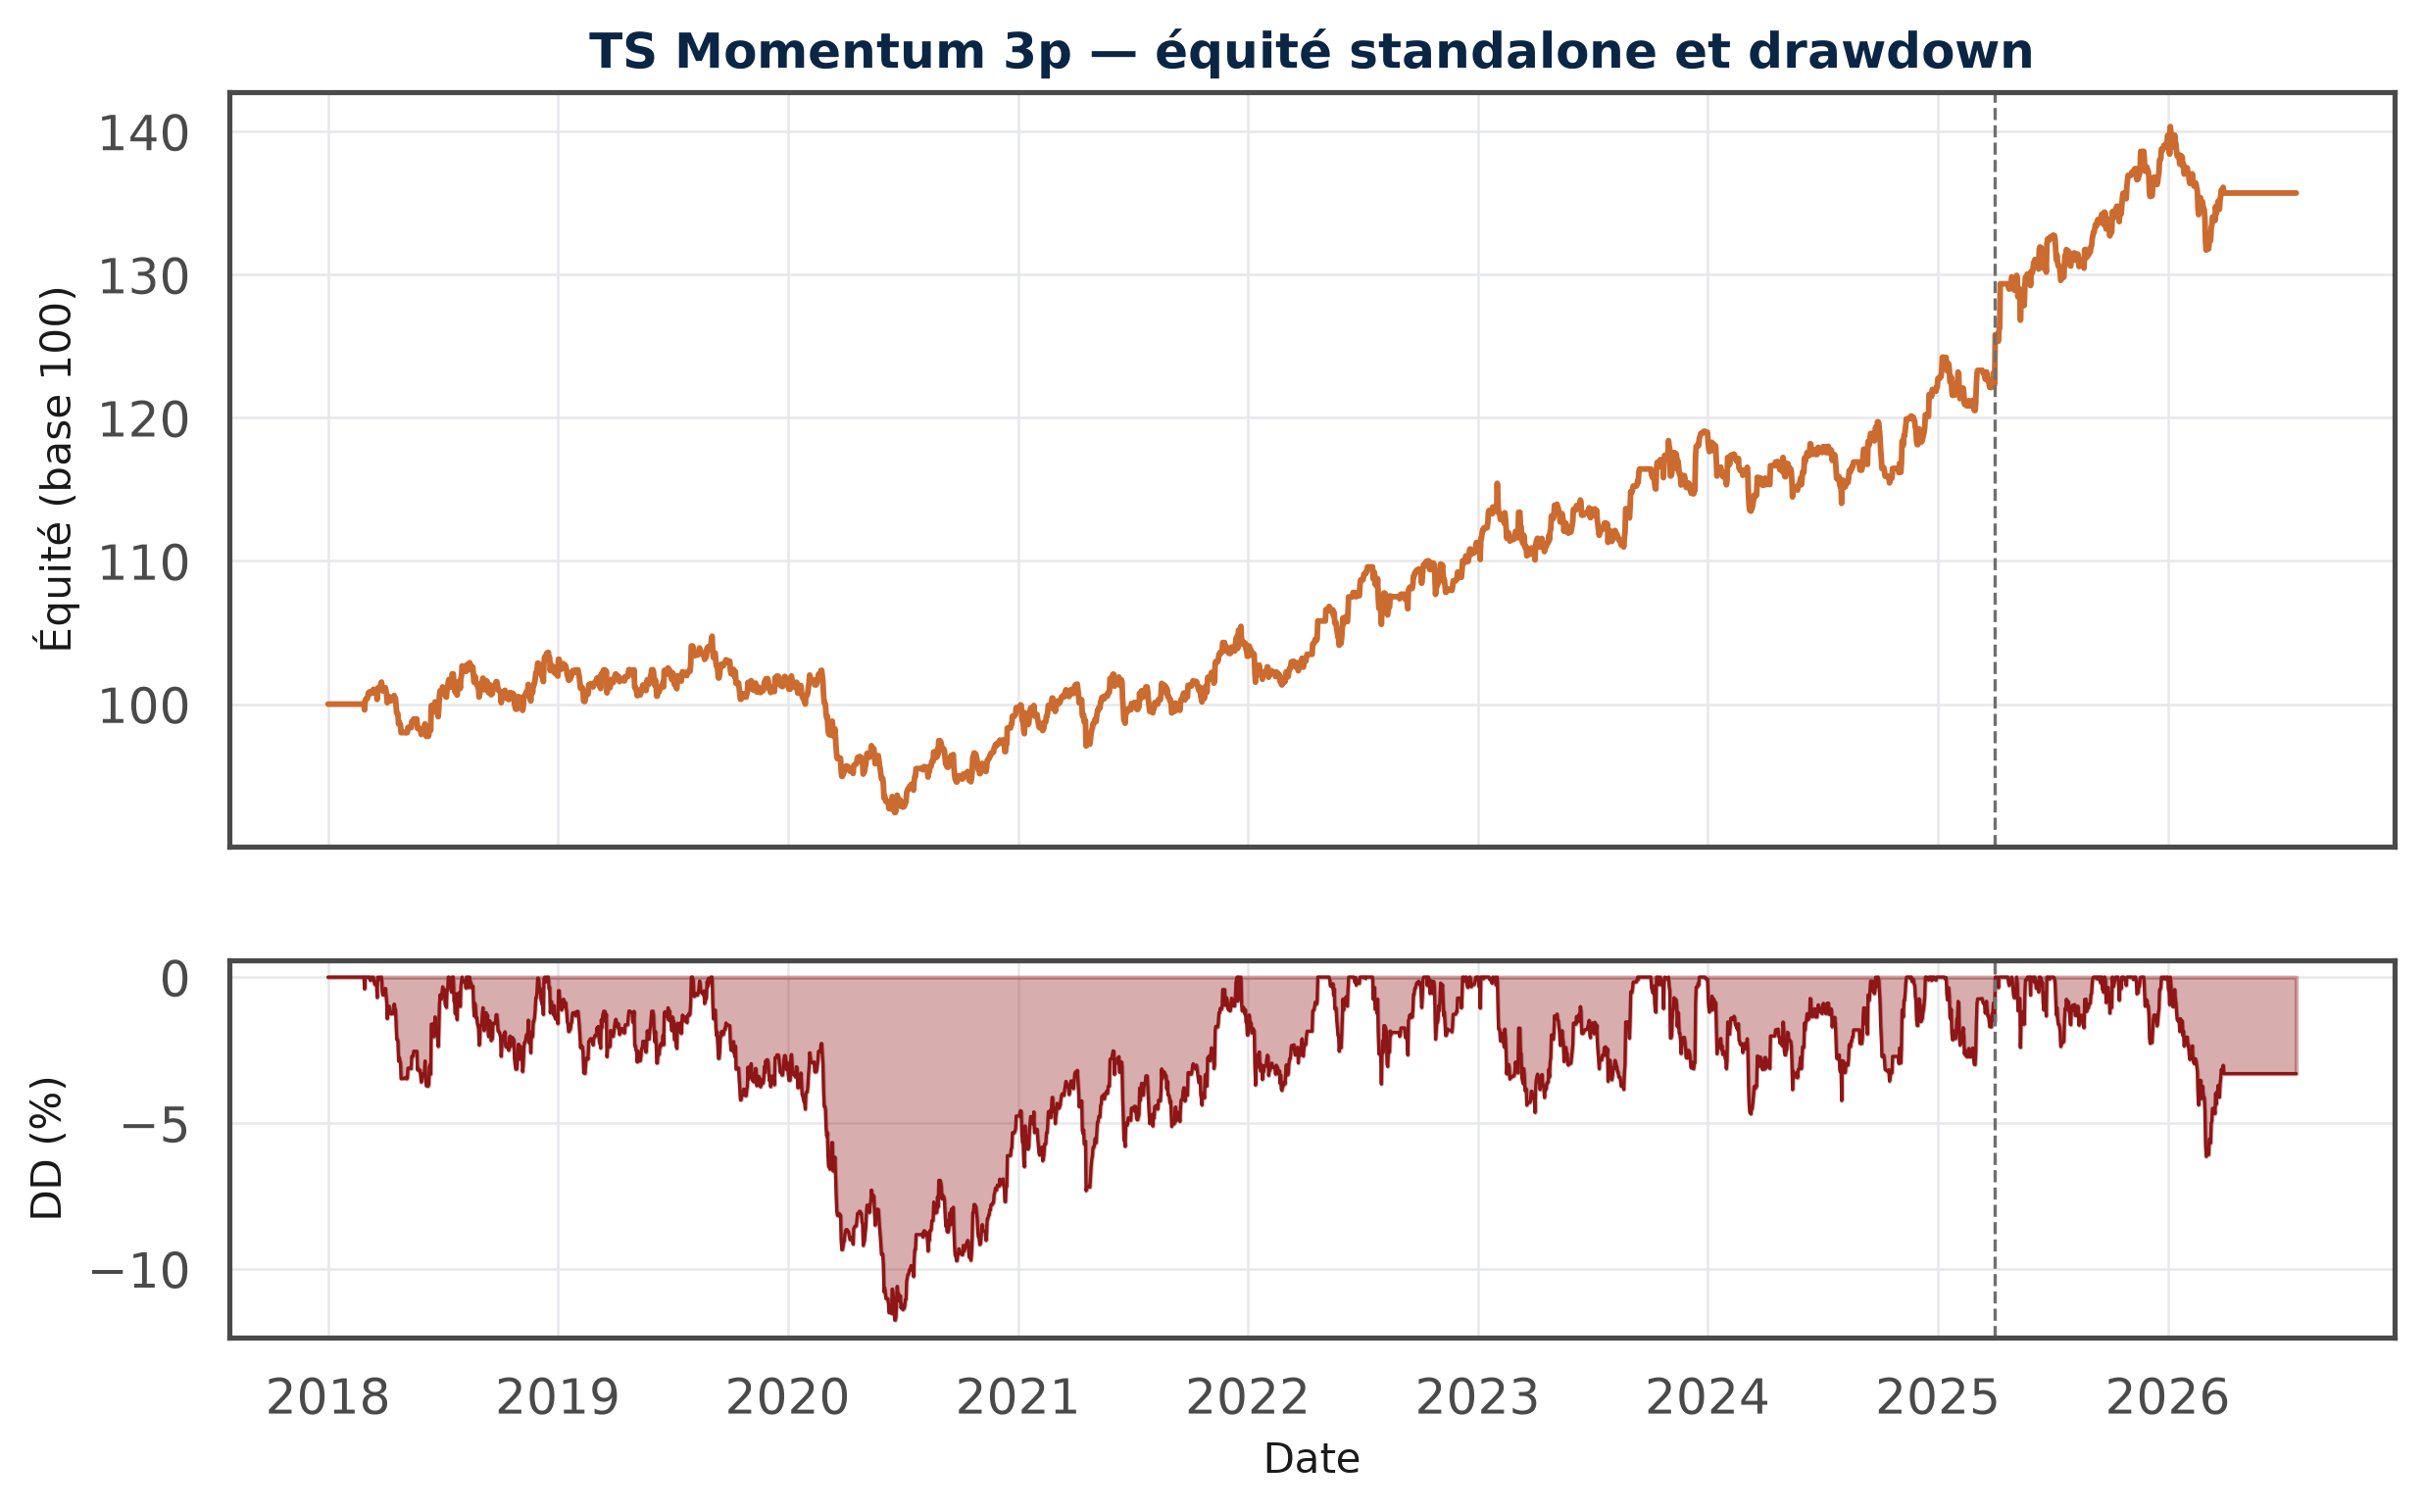
\includegraphics[width=\linewidth]{sleeve_ts_momentum_3p_equity.png}
\caption{Équité et drawdown du Moteur~2 (trois paires) pris isolément.}
\end{figure}

\begin{insightbox}
\textbf{Le Moteur~2 est le contributeur principal de la performance hors
échantillon.} Sur la fenêtre de validation 2025-04 à 2026-04, son Sharpe atteint
$1{,}26$, bien au-dessus de son Sharpe \emph{full-period} de $0{,}57$. Cela
suggère que les régimes monétaires récents (divergence Fed/BCE/BoJ) sont
particulièrement favorables au suivi de tendance FX. Conclusion~: maintenir un
moteur de tendance dans le portefeuille même lorsque son Sharpe in-sample paraît
modeste, car son rôle se révèle exactement quand on en a besoin.
\end{insightbox}

\newpage

% ═══════════════════════════════════════════════════════════════════════
%  § 5 — MOTEUR 3 : RSI DAILY
% ═══════════════════════════════════════════════════════════════════════
\section{Moteur 3 --- RSI Daily (mean reversion swing)}
\label{sec:rsi_daily}

\subsection{Intuition économique}

\begin{thesisbox}
\textbf{Un mouvement directionnel exacerbé sur une journée est un \emph{overshoot}
statistiquement rare.} Lorsque l'indicateur RSI journalier d'une paire FX
majeure dépasse $75$ (sur-achat) ou descend sous $25$ (sur-vente), il reflète
une accumulation disproportionnée de flux dans une seule direction~--- typiquement
déclenchée par une annonce macroéconomique ou un \emph{squeeze} technique.
L'expérience empirique montre que ces extrêmes se résolvent en 2~à 10~jours
par un retour du prix vers un RSI neutre autour de $50$.
\end{thesisbox}

Ce moteur exploite \emph{exactement le régime opposé} à celui du Moteur~2~: là où le suivi de tendance capture les mouvements lents déployés sur plusieurs semaines, le RSI Daily capture les excès de court terme. C'est de cette opposition stylistique que naît la corrélation négative observée ($-0{,}25$ sur la période complète) entre les deux moteurs, qui est le levier central de la diversification.

\subsection{Mécanique du signal}

\begin{enumerate}
\item \textbf{Calcul du RSI(14)} sur le close journalier de chaque paire.
\item \textbf{Détection de croisement} sur deux jours consécutifs (\texttt{shift~=~1} et \texttt{shift~=~2})~:
  \begin{itemize}
  \item Long si la veille le RSI est passé sous $25$ (la veille $\geq 25$, aujourd'hui $< 25$).
  \item Short si la veille le RSI est passé au-dessus de $75$ (la veille $\leq 75$, aujourd'hui $> 75$).
  \end{itemize}
\item \textbf{Sortie sur croisement de retour} vers $50$ (RSI neutre).
\item \textbf{Time-stop à $21$ jours} : si la position est encore ouverte après trois semaines, on ferme. Cette règle limite l'accumulation de \emph{swap} (intérêts overnight) lorsque le RSI oscille autour de $50$ sans franchissement net.
\item \textbf{Univers} : EUR/USD, GBP/USD, USD/CAD (pas USD/JPY). Le retrait de USD/JPY a été démontré bénéfique sur l'historique~: le \emph{swap} négatif sur cette paire ronge l'edge du moteur.
\end{enumerate}

\subsection{Le paradoxe du Sharpe individuel}

\begin{warningbox}
\textbf{Le Moteur~3 a un Sharpe \emph{standalone} d'environ $0{,}16$ sur la période
complète.} C'est de loin le plus faible des trois. Pourtant, son retrait ferait
perdre environ $30\,\%$ du Sharpe du portefeuille combiné. C'est la définition
exacte d'un diversificateur anti-corrélé de valeur.
\end{warningbox}

La décomposition année par année révèle le mécanisme~:

\begin{center}
\renewcommand{\arraystretch}{1.1}
\begin{tabular}{lrrr p{4cm}}
\toprule
\textbf{Année} & \textbf{Moteur 3} & \textbf{Moteur 1} & \textbf{Moteur 2} & \textbf{Commentaire} \\
\midrule
2019 & \textcolor{rsiGreen}{$+0{,}95\,\star$} & $-0{,}64$ & $-0{,}41$ & Le Moteur~3 sauve l'année \\
2020 & $-0{,}03$ & $+1{,}19$ & $-0{,}24$ & --- \\
2021 & $+0{,}61$ & $0{,}00$ & $+0{,}62$ & --- \\
2022 & $-0{,}51$ & \textcolor{rsiGreen}{$+2{,}23$} & $+1{,}18$ & --- \\
2023 & \textcolor{rsiGreen}{$+0{,}92\,\star$} & $-0{,}28$ & $+0{,}55$ & Le Moteur~3 sauve l'année \\
2024 & $-0{,}24$ & $+2{,}08$ & $+0{,}61$ & --- \\
2025 & $+0{,}38$ & $+0{,}72$ & $+1{,}57$ & --- \\
2026 YTD & \textcolor{rsiGreen}{$+3{,}54\,\star$} & $+1{,}72$ & $-1{,}59$ & Le Moteur~3 sauve le YTD \\
\bottomrule
\end{tabular}
\end{center}

\textbf{Le Moteur~3 est positif exactement dans les années où les deux autres perdent.} La matrice de corrélation confirme cette anti-corrélation~:

\[
\begin{array}{l|rrr}
 & \text{Moteur 1} & \text{Moteur 2} & \text{Moteur 3} \\
\hline
\text{Moteur 1} & 1{,}000  & +0{,}056 & -0{,}027 \\
\text{Moteur 2} & +0{,}056 & 1{,}000  & \mathbf{-0{,}251} \\
\text{Moteur 3} & -0{,}027 & \mathbf{-0{,}251} & 1{,}000 \\
\end{array}
\]

\subsection{Paramètres expliqués}

\begin{center}
\renewcommand{\arraystretch}{1.3}
\small
\begin{tabular}{p{3.4cm}p{1.8cm}p{8.2cm}}
\toprule
\textbf{Paramètre} & \textbf{Valeur} & \textbf{Pourquoi cette valeur ?} \\
\midrule
\code{Inp\_RSI\_Period} & $14$ & Période standard de Wilder. Capture la dynamique journalière sans sur-réagir aux \emph{spikes} d'un seul jour. \\
\code{Inp\_RSI\_Oversold} & $25$ & Seuil long. Plus strict que le $30$ classique : on ne trade que les vrais extrêmes. \\
\code{Inp\_RSI\_Overbought} & $75$ & Seuil short. Symétrique du précédent. \\
\code{Inp\_RSI\_ExitMid} & $50$ & Niveau RSI déclenchant la sortie. Le retour à $50$ marque la fin de l'\emph{overshoot} et le retour à un régime neutre. \\
\code{Inp\_RSI\_TimeStopDays} & $21$ & Durée maximale de détention. Au-delà de trois semaines, le \emph{swap} cumulé annule l'edge du signal~: on ferme. \\
\bottomrule
\end{tabular}
\end{center}

\subsection{Performance historique}

\begin{figure}[H]
\centering

\includegraphics[width=\linewidth]{sleeve_rsi_daily_3p_equity.png}
\caption{Équité du Moteur~3 pris isolément. Courbe relativement plate, avec des pics positifs en 2019, 2023 et début 2026 qui correspondent exactement aux années faibles des autres moteurs~--- profil typique d'un diversificateur.}
\end{figure}

\begin{insightbox}
\textbf{La leçon de construction de portefeuille~:} un moteur à Sharpe individuel
faible peut être le meilleur diversificateur si sa corrélation avec le reste
est négative dans les années difficiles. Ce qui compte n'est pas le Sharpe
isolé mais la \textbf{contribution marginale au Sharpe combiné}, qui dépend
directement de la corrélation. Un signal à Sharpe $0{,}16$ anti-corrélé bat
fréquemment un signal à Sharpe $0{,}60$ fortement corrélé.
\end{insightbox}

\newpage

% ═══════════════════════════════════════════════════════════════════════
%  § 6 — MOTEUR 4 : GOLD MOMENTUM
% ═══════════════════════════════════════════════════════════════════════
\section{Moteur 4 --- Gold Momentum (suivi de tendance sur l'or)}
\label{sec:gold}

\subsection{Intuition économique}

Les trois premiers moteurs travaillent sur des paires de devises. Le quatrième
travaille sur l'or (\code{XAUUSD}), et exploite une régularité différente~: le
\emph{time series momentum}. Documentée par Moskowitz, Ooi et Pedersen
(\emph{Journal of Financial Economics}, 2012) sur plus de cinquante marchés à
terme, elle énonce que le rendement passé d'un actif prédit son rendement futur
sur des horizons de un à douze mois.

L'or est un terrain naturel pour cette anomalie. Il ne verse pas de coupon et ne
génère pas de flux~: son prix est presque entièrement porté par des flux de
capitaux et des changements de régime macroéconomique~--- inflation anticipée,
taux réels, aversion au risque. Ces changements se propagent lentement, ce qui
crée des tendances de plusieurs semaines à plusieurs mois plutôt que des
retournements rapides.

C'est aussi, et c'est le point qui justifie sa présence, une source de rendement
\textbf{structurellement décorrélée} des trois moteurs FX. Ceux-ci vivent des
divergences de politique monétaire entre banques centrales et de la
micro-structure du marché des changes. L'or répond à autre chose.

\subsection{Mécanique du signal}

Le piège classique du \emph{momentum} est le choix de l'horizon~: retenir la
fenêtre qui a le mieux marché sur l'historique revient à sur-ajuster. Ce moteur
l'évite en \textbf{refusant de choisir}.

\begin{enumerate}
\item Quatre horizons fixes sont évalués en parallèle~: $40$, $60$, $120$ et
      $250$~séances.
\item Pour chacun, on ne retient que le \emph{signe} du rendement passé~--- pas
      son amplitude, qui serait bien plus bruitée.
\item Les quatre signes sont moyennés. Le résultat est un signal d'ensemble.
\item La position s'ouvre quand l'ensemble devient positif et se ferme quand il
      redevient négatif.
\end{enumerate}

Moyenner remplace un choix par un agrégat. C'est à la fois plus proche de la
manière dont la littérature applique le TSMOM en pratique, et nettement plus
difficile à sur-ajuster~: aucun des quatre horizons n'a été optimisé.

\begin{insightbox}
\textbf{Le moteur est \emph{long-only}.} Il n'y a pas de vente à découvert sur
l'or (\code{Inp\_Gold\_AllowShort = false}). Quand l'ensemble est négatif, le
moteur est simplement hors marché. Ce choix supprime la queue de risque la plus
brutale~--- un \emph{short squeeze} sur l'or~--- au prix des tendances baissières
non exploitées.
\end{insightbox}

Les positions se comptent en semaines, pas en heures~: sur la fenêtre de
référence de cinq ans et quatre mois, le moteur n'a ouvert que \textbf{35~positions}.
C'est de loin le moteur le moins actif du portefeuille, et c'est cohérent avec un
signal d'horizon long.

\subsection{Paramètres expliqués}

\begin{center}
\renewcommand{\arraystretch}{1.3}
\small
\begin{tabular}{p{3.9cm}p{1.8cm}p{7.7cm}}
\toprule
\textbf{Paramètre} & \textbf{Valeur} & \textbf{Pourquoi cette valeur ?} \\
\midrule
\code{Inp\_Gold\_Symbol} & \texttt{XAUUSD} & Le symbole or du broker. Le suffixe de compte (\code{.c}) est ajouté automatiquement. \\
\code{Inp\_Gold\_LookbackA..D} & $40/60/120/250$ & Les quatre horizons de l'ensemble, en séances. Fixés a priori depuis la littérature TSMOM, jamais optimisés. \\
\code{Inp\_Gold\_AllowShort} & \texttt{false} & Long-only. Voir l'encadré ci-dessus. \\
\code{Inp\_Gold\_TargetVol} & $0{,}55$ & Volatilité annualisée visée pour ce moteur pris isolément. Élevée par construction~: c'est un moteur de rendement, borné en aval par son allocation de $10\,\%$. \\
\code{Inp\_Gold\_MaxLeverage} & $6{,}6$ & Plafond de levier propre au moteur, qui borne l'exposition quand la volatilité réalisée de l'or s'effondre. \\
\code{Inp\_Gold\_SafetySL} & $0{,}04$ & Stop de sécurité à $4\,\%$ du prix d'entrée. Ce n'est pas un stop de stratégie~--- le signal sort de lui-même~--- mais un garde-fou contre un décrochage brutal. \\
\code{Inp\_Gold\_SlippageBps} & $2$ & Slippage modélisé, en points de base par côté. Plus bas que sur les paires FX~: le marché de l'or spot est profond aux volumes traités ici. \\
\bottomrule
\end{tabular}
\end{center}

\subsection{Performance historique}

\begin{figure}[H]
\centering

\includegraphics[width=\linewidth]{sleeve_gold_momentum_equity.png}
\caption{Équité du Moteur~4 pris isolément, à son dimensionnement propre et \emph{avant} l'allocation de $10\,\%$. La progression est très irrégulière~: de longues périodes hors marché ou sans progrès, ponctuées de quelques mouvements de grande amplitude qui font l'essentiel du résultat.}
\end{figure}

Pris isolément et à son dimensionnement propre, le moteur rend $577{,}8\,\%$ sur
la période, soit un CAGR de $25{,}06\,\%$, pour une volatilité annualisée de
$33{,}88\,\%$ et un Sharpe de $0{,}74$. Son repli maximal isolé atteint
$-79{,}62\,\%$.

\begin{warningbox}
\textbf{Ce moteur porte le résultat, et il porte le risque.} Sur le backtest
d'exécution MetaTrader~5 de référence, il produit $79{,}8\,\%$ du profit net du
portefeuille avec $10\,\%$ de l'allocation et $4\,\%$ des transactions. Son taux
de réussite est de $31{,}4\,\%$~: environ deux positions sur trois perdent de
l'argent, et l'ensemble du résultat vient d'une minorité de mouvements longs.

\smallskip
Trois conséquences pratiques qu'il faut avoir en tête avant de déployer~:
\begin{itemize}
\item \textbf{Une longue série de pertes est le régime normal}, pas un signal de
      dysfonctionnement. Un moteur de suivi de tendance à $31\,\%$ de réussite
      passe l'essentiel de son temps à perdre de petites sommes.
\item \textbf{La performance du portefeuille est concentrée.} Si l'or entre dans
      un régime sans tendance durable, le portefeuille perd sa principale source
      de rendement et retombe sur les trois moteurs FX, dont les CAGR isolés
      s'échelonnent entre $1{,}5\,\%$ et $5{,}2\,\%$~--- un tout autre ordre de
      grandeur.
\item \textbf{Le repli isolé de $-79{,}62\,\%$ est réel}, même s'il est ramené à
      l'échelle du portefeuille par l'allocation de $10\,\%$ et par la couche de
      ciblage de volatilité globale.
\end{itemize}
\end{warningbox}

\begin{insightbox}
\textbf{Pourquoi $10\,\%$ et pas davantage~?} Parce que le poids optimal apparent
de ce moteur se situe à la borne du domaine testé~--- autrement dit, les données
disponibles ne permettent pas de trancher entre $10\,\%$ et une valeur plus
élevée. Face à une indétermination de ce type, le choix retenu est le plus
prudent des deux. Augmenter cette part serait une décision à prendre sur des
données futures, pas sur celles qui ont servi à la calibrer.
\end{insightbox}

\newpage

% ═══════════════════════════════════════════════════════════════════════
%  § 7 — GESTION DU RISQUE
% ═══════════════════════════════════════════════════════════════════════
\section{Gestion du risque}
\label{sec:risk}

La couche de risque s'applique uniformément aux quatre moteurs et constitue la \emph{moitié invisible} de la stratégie~: elle ne génère pas de signal, mais elle modère, plafonne et protège.

\subsection{Ciblage de volatilité global}

Chaque jour à 21h~UTC, après la fermeture des positions intraday du Moteur~1, la couche de risque recalcule un \textbf{levier global} commun aux quatre moteurs. La formule~:

\[
\text{leverage} = \min\!\left(\frac{\text{target\_vol}}{\max(\sigma_{21},\,\sigma_{63},\,\text{vol\_floor})},\ \text{max\_leverage}\right)
\]

où~:
\begin{itemize}
\item $\sigma_{21}$ est la volatilité réalisée du portefeuille sur 21 jours,
\item $\sigma_{63}$ idem sur 63 jours,
\item $\text{target\_vol} = 0{,}75$ (la cible),
\item $\text{vol\_floor} = 0{,}02$ (plancher pour éviter une division par zéro),
\item $\text{max\_leverage} = 31$ (plafond dur).
\end{itemize}

\begin{insightbox}
\textbf{Pourquoi le maximum entre $\sigma_{21}$ et $\sigma_{63}$ ?} Pour rester
conservateur. Si la volatilité récente est plus élevée que la volatilité longue,
on prend $\sigma_{21}$ et on déleverage. Si la volatilité récente est plus basse
(régime calme), on prend $\sigma_{63}$ et on évite de \emph{maxer} le levier
juste avant un retour de la volatilité. C'est une asymétrie volontaire en
faveur du risque baissier.
\end{insightbox}

\subsection{Disjoncteur de drawdown (DD-cap)}

\begin{warningbox}
\textbf{Le \emph{DD-cap} est un \emph{garde-fou}, pas un \emph{outil de trading}.}
S'il se déclenche, c'est qu'il faut auditer~: comprendre ce qui s'est passé,
vérifier l'intégrité des données, et décider manuellement de réactiver ou non
la stratégie.
\end{warningbox}

\textbf{Ce disjoncteur est désactivé dans la configuration livrée} (\code{Inp\_EnableDDCap = false}). Le mandat ne fixant plus de plafond de repli, il n'a aucun seuil à faire respecter~; les tests avaient par ailleurs montré qu'il dégradait la performance en réduisant l'exposition pendant les phases de rebond.

\textbf{Il n'existe donc aucun coupe-circuit automatique.} Le repli d'équité constaté sur le backtest de référence atteint $44\,\%$, et rien ne l'aurait interrompu s'il était allé plus loin. C'est un choix assumé du mandant, pas un oubli.

Le mécanisme reste disponible et peut être réactivé à tout moment~: en le passant à \code{true}, la couche de risque compare chaque seconde l'\emph{equity} courante au plus haut historique et ferme toutes les positions si le repli dépasse le seuil \code{Inp\_DDCap} ($20\,\%$ par défaut), en armant un verrou que seul un \emph{reset} manuel lève.

\subsection{Plafond d'utilisation de la marge}
\label{sec:margin_cap}

Contrairement au disjoncteur de \emph{drawdown}, ce mécanisme-ci est \textbf{actif par défaut} (\code{Inp\_EnableMarginCap = true}). Indépendamment du \emph{drawdown} en P\&L, la marge engagée auprès du broker est surveillée toutes les 30~secondes. Deux seuils~:

\begin{itemize}
\item \textbf{$50\,\%$ de marge utilisée}~: le levier global est divisé par deux. Effet immédiat sur les nouvelles entrées (sizing réduit), pas de fermeture forcée.
\item \textbf{$85\,\%$ de marge utilisée}~: \textbf{fermeture forcée immédiate} de toutes les positions. Niveau d'urgence avant un \emph{margin call} broker, qui se déclencherait typiquement vers $90\,\%$--$100\,\%$.
\end{itemize}

\subsection{Filtre des fenêtres de news}

Cette protection est spécifique au Moteur~1 (intraday). Elle interroge le calendrier économique MetaTrader pour identifier les publications USD \enquote{high impact} (NFP, CPI, FOMC, retail sales, GDP, \ldots) et bloque toute nouvelle entrée dans une fenêtre de $\pm 15$~minutes autour de chaque publication.

\begin{examplebox}
\textbf{Pourquoi $\pm 15$~minutes et pas $\pm 5$ ?} Parce que le \emph{spread}
typique sur EUR/USD passe de $1$ pip à $8$--$10$ pips dans les minutes qui
encadrent un NFP, et qu'il met plusieurs minutes après le pic à revenir à un
niveau normal. Une fenêtre étroite à $\pm 5$~min laisserait passer des trades
exécutés sur un \emph{spread} encore élargi de $3$--$5$ pips, érodant l'edge.
\end{examplebox}

\subsection{Hiérarchie des protections}

Les quatre disjoncteurs s'enchaînent de la moins agressive à la plus agressive~:

\begin{enumerate}
\item \textbf{Filtre news} : prévention pure, refuse les entrées dangereuses.
\item \textbf{Vol-targeting} : modère la taille des positions selon le régime.
\item \textbf{Margin-cap} : réduit le levier ou ferme tout selon la marge.
\item \textbf{DD-cap} : ferme tout en cas de pertes cumulées graves, requiert un \emph{reset} manuel.
\end{enumerate}

Cette hiérarchie est volontairement \emph{conservatrice et redondante}~: chaque couche peut compenser une défaillance de la précédente.

\newpage

% ═══════════════════════════════════════════════════════════════════════
%  § 7 — COÛTS D'EXÉCUTION
% ═══════════════════════════════════════════════════════════════════════
\section{Coûts d'exécution réalistes}
\label{sec:costs}

Une stratégie quantitative qui ignore les frais réels est une stratégie qui sur-estime son edge. La modélisation des coûts dans FxMultiSleeve est conservative et calibrée sur les pratiques observées chez les brokers ECN/STP utilisés en production.

\subsection{Slippage}

Le \emph{slippage} est l'écart entre le prix anticipé et le prix d'exécution réel. Sur les ordres au marché, il provient de la latence réseau, du décalage tick et de la profondeur du carnet d'ordres.

\begin{center}
\renewcommand{\arraystretch}{1.2}
\begin{tabular}{lrr}
\toprule
\textbf{Moteur} & \textbf{Slippage par côté} & \textbf{Round-trip} \\
\midrule
Moteur 1 (MR Macro, intraday) & $15$ bps & $30$ bps \\
Moteur 2 (TS Momentum, daily) & $10$ bps & $20$ bps \\
Moteur 3 (RSI Daily, daily)   & $10$ bps & $20$ bps \\
\bottomrule
\end{tabular}
\end{center}

Ces valeurs sont \emph{plus conservatrices} que les valeurs typiques observées sur EUR/USD chez OANDA Core, IC~Markets Raw ou Pepperstone Razor, qui se situent plutôt vers $5$--$10$~bps par côté en conditions normales. Le surcoût modélisé absorbe les \emph{spikes} occasionnels et garde une marge de sécurité.

\paragraph{Application technique.}
Le slippage est appliqué de deux manières dans la stratégie~:
\begin{enumerate}
\item Décalage des niveaux SL et TP par \texttt{slip\_pct} pour absorber le coût des sorties par stop ou take-profit.
\item Pré-paiement via une réduction proportionnelle du \emph{sizing} (\texttt{slip\_drag}) pour couvrir les sorties \enquote{non-déclenchées} (time-stop, fermeture quotidienne, inversion de signal).
\end{enumerate}

\subsection{Commission}

\begin{center}
\renewcommand{\arraystretch}{1.2}
\begin{tabular}{lll}
\toprule
\textbf{Type de compte} & \textbf{Commission} & \textbf{Équivalent EUR/USD} \\
\midrule
OANDA Standard & $0$ commission, \emph{spread-only} & --- \\
OANDA Core / IC Markets Raw & $\sim \$5$ par lot par côté & $\sim 4{,}5$ bps \\
Pepperstone Razor & $\sim \$3{,}5$ par lot par côté & $\sim 3{,}2$ bps \\
\bottomrule
\end{tabular}
\end{center}

La stratégie modélise par défaut $5$ bps de commission par côté (\code{Inp\_CommissionBpsPerSide=5{,}0}), correspondant à un compte de type Core / Raw. Si vous opérez sur un compte \emph{spread-only} (OANDA Standard), passez ce paramètre à $0$.

\subsection{Swap rollover}

Toute position détenue à la clôture du marché à 22h~UTC subit un débit ou crédit \emph{swap}, calculé par le broker en fonction du différentiel de taux d'intérêt entre les deux devises de la paire.

\begin{itemize}
\item \textbf{Modélisation par défaut} : $0{,}5$ bps par nuit (\code{Inp\_SwapBpsPerNight=0{,}5}), soit environ $\$1{,}50$ par 100\,000~EUR détenu une nuit.
\item Cette valeur est conservatrice~: certaines paires en \emph{carry positif} (USD/JPY long avant 2024) génèrent un swap positif, d'autres en \emph{carry négatif} (EUR/USD short en cycle de hausse Fed) coûtent davantage. La modélisation absolue à $0{,}5$ bps absorbe le pire cas.
\item Le Moteur~1 est intraday et ne paie jamais de swap. Les Moteurs~2 et~3 paient sur leurs détentions multi-jours.
\end{itemize}

\subsection{Spread spike news}

Lors des publications \enquote{high impact} (NFP, CPI, FOMC), le \emph{spread} EUR/USD typique passe de $1$ pip à $8$--$10$ pips pendant 1 à 5 minutes. Cette élargissement transitoire peut détruire un trade quasi-instantanément.

\begin{warningbox}
\textbf{Le filtre de news (\S~\ref{sec:risk}) est précisément là pour mitiger ce
risque.} Sans filtre, sur une fenêtre de cinq ans, l'érosion estimée de la
performance par les \emph{spread spikes} approche $10\,\%$ du P\&L net du
Moteur~1.
\end{warningbox}

\subsection{Contribution totale des frais}

Sur la fenêtre de validation 2020-11 à 2026-04 (5{,}4~ans), la décomposition des coûts du portefeuille combiné~:

\begin{center}
\renewcommand{\arraystretch}{1.2}
\begin{tabular}{lr}
\toprule
\textbf{Poste} & \textbf{Total} \\
\midrule
Commission (5 bps/côté) & pré-payé via décalage SL/TP \\
Swap rollover cumulé    & $\sim -410$ USD \\
Slippage round-trip     & absorbé via décalage SL/TP \\
\midrule
\textbf{Net} & \textbf{réalité broker reflétée} \\
\bottomrule
\end{tabular}
\end{center}

Le \emph{swap} est concentré sur les Moteurs~2 et~3 ($-408$ USD à eux deux) ; le Moteur~1 (intraday) le ramène à zéro. Sur un capital initial de \$10\,000, $\$410$ de swap sur 5{,}4~ans représente un drag annuel de l'ordre de $0{,}8\,\%$~--- significatif mais maîtrisé.

\newpage

% ═══════════════════════════════════════════════════════════════════════
%  § 8 — PARAMÈTRES : RÉFÉRENCE COMPLÈTE
% ═══════════════════════════════════════════════════════════════════════
\section{Paramètres : référence complète}
\label{sec:params}

Cette section consolide l'ensemble des paramètres modifiables, organisés par groupe fonctionnel. Pour chaque paramètre~: la valeur par défaut, la justification, et le scénario qui appellerait à le modifier.

\subsection{Allocation et risque}

\begin{center}
\renewcommand{\arraystretch}{1.3}
\small
\begin{tabular}{p{3.6cm}p{1.4cm}p{8.5cm}}
\toprule
\textbf{Paramètre} & \textbf{Défaut} & \textbf{Quand le toucher ?} \\
\midrule
\code{Inp\_AllocMRMacro}      & $0{,}72$  & Jamais (sauf rééquilibrage stratégique majeur). \\
\code{Inp\_AllocTSMomentum}   & $0{,}09$  & Jamais. \\
\code{Inp\_AllocRSIDaily}     & $0{,}09$  & Jamais. \\
\code{Inp\_AllocGoldMomentum} & $0{,}10$  & Jamais. La somme des quatre allocations doit valoir exactement $1{,}0$. \\
\code{Inp\_RiskScale}         & $4{,}5$   & \textbf{Le réglage du risque}. Rendement et repli y répondent proportionnellement~: l'abaisser réduit les deux, sans changer les signaux ni le nombre de trades. \\
\code{Inp\_EnableDDCap}       & \texttt{false} & Désactivé dans la configuration livrée. À passer à \texttt{true} pour réactiver le coupe-circuit de repli. \\
\code{Inp\_DDCap}             & $0{,}20$  & Seuil du coupe-circuit, utilisé uniquement si \code{Inp\_EnableDDCap} vaut \texttt{true}. \\
\code{Inp\_EnableMarginCap}   & \texttt{true} & \textbf{Actif.} Jamais déclenché en backtest, mais il protège en conditions réelles (cf.~\ref{sec:margin_cap}). \\
\code{Inp\_MarginCapPct}      & $0{,}50$  & Seuil de déclenchement du désendettement. À adapter selon la marge dont vous disposez en réserve. \\
\bottomrule
\end{tabular}
\end{center}

\subsection{Vol-targeting global}

\begin{center}
\renewcommand{\arraystretch}{1.3}
\small
\begin{tabular}{p{3.6cm}p{1.4cm}p{8.5cm}}
\toprule
\textbf{Paramètre} & \textbf{Défaut} & \textbf{Quand le toucher ?} \\
\midrule
\code{Inp\_GlobalTargetVol}    & $0{,}37$ & Cible de volatilité du portefeuille. À réduire sur un compte EU retail plafonné à $30\times$. \\
\code{Inp\_GlobalMaxLeverage}  & $31{,}0$ & Plafond levier. À ajuster au levier maximum offert par votre broker. \\
\code{Inp\_GlobalVolFloor}     & $0{,}02$ & Plancher anti-zéro. Ne pas modifier. \\
\bottomrule
\end{tabular}
\end{center}

\subsection{Coûts d'exécution}

\begin{center}
\renewcommand{\arraystretch}{1.3}
\small
\begin{tabular}{p{3.8cm}p{1.4cm}p{8.3cm}}
\toprule
\textbf{Paramètre} & \textbf{Défaut} & \textbf{Quand le toucher ?} \\
\midrule
\code{Inp\_MR\_SlippageBps}        & $15$ & Si votre broker affiche un \emph{spread} typique très différent de la moyenne (voir \S~\ref{sec:costs}). \\
\code{Inp\_TS\_SlippageBps}        & $10$ & Idem. \\
\code{Inp\_RSI\_SlippageBps}       & $10$ & Idem. \\
\code{Inp\_CommissionBpsPerSide}   & $5{,}0$ & Mettre à $0$ sur compte \emph{spread-only}. Mettre à $3{,}5$ sur Pepperstone Razor / IC~Markets Raw. \\
\code{Inp\_SwapBpsPerNight}        & $0{,}5$ & Augmenter si le broker pratique des swaps particulièrement défavorables. \\
\bottomrule
\end{tabular}
\end{center}

\subsection{Source des données macro}

\begin{center}
\renewcommand{\arraystretch}{1.3}
\small
\begin{tabular}{p{4.0cm}p{1.6cm}p{7.9cm}}
\toprule
\textbf{Paramètre} & \textbf{Défaut} & \textbf{Quand le toucher ?} \\
\midrule
\code{Inp\_MacroSourceMode}        & \code{AUTO} & \emph{AUTO} sélectionne automatiquement HISTORY en backtest, NATIVE en live. Ne pas changer sauf cas particulier. \\
\code{Inp\_MR\_SpreadThresh}       & $0{,}5$ & Seuil 10Y-2Y pour le filtre macro. À ne pas relâcher sans tests~: trop large détruit l'edge. \\
\code{Inp\_MR\_NewsFilterEnabled}  & \texttt{true} & Garder activé en production. À désactiver uniquement pour mesurer l'impact du filtre. \\
\code{Inp\_FREDApiKeyFile}         & \texttt{fred\_api\_key.txt} & Nom du fichier contenant votre clé FRED. Voir \emph{Guide d'installation}. \\
\code{Inp\_MacroHistoryFile}       & \texttt{macro\_history.csv} & Nom du CSV utilisé en backtest. Voir \emph{Guide d'installation}. \\
\bottomrule
\end{tabular}
\end{center}

\subsection{Opérationnel}

\begin{center}
\renewcommand{\arraystretch}{1.3}
\small
\begin{tabular}{p{3.6cm}p{2.0cm}p{7.8cm}}
\toprule
\textbf{Paramètre} & \textbf{Défaut} & \textbf{Quand le toucher ?} \\
\midrule
\code{Inp\_SymbolSuffix} & \texttt{".c"} & \textbf{À adapter au broker.} Exemples~: \texttt{""}, \texttt{".m"}, \texttt{".raw"}, \texttt{"-pro"}. Vérifier dans MarketWatch. \\
\code{Inp\_MagicMR}      & $831$  & Identifiant des positions du Moteur~1. Ne pas modifier sauf collision avec un autre EA. \\
\code{Inp\_MagicTS}      & $832$  & Idem Moteur~2. \\
\code{Inp\_MagicRSI}     & $833$  & Idem Moteur~3. \\
\code{Inp\_LogVerbose}   & \texttt{false} & Mettre à \texttt{true} pour debug détaillé. Coûteux en performance. \\
\code{Inp\_LogToFile}    & \texttt{true}  & Garder activé pour l'audit. \\
\code{Inp\_ExportDeals}  & \texttt{false} & Activer pour un run d'analyse trade par trade ; coûteux donc à laisser éteint en production. \\
\bottomrule
\end{tabular}
\end{center}

\newpage

% ═══════════════════════════════════════════════════════════════════════
%  § 9 — LECTURE DES RÉSULTATS BACKTEST
% ═══════════════════════════════════════════════════════════════════════
\section{Lecture des résultats backtest}
\label{sec:reading_results}

À chaque exécution, le moteur émet un rapport HTML standard MetaTrader et un dump JSON structuré. Voici comment interpréter les principales métriques.

\subsection{Métriques de premier ordre}

\begin{center}
\renewcommand{\arraystretch}{1.3}
\small
\begin{tabular}{p{3.4cm}p{2.3cm}p{8.5cm}}
\toprule
\textbf{Métrique} & \textbf{Cible} & \textbf{Lecture} \\
\midrule
Sharpe ratio (rf=0) & $> 1{,}0$ acceptable, $> 1{,}5$ excellent & Rendement annualisé divisé par volatilité annualisée. Mesure l'efficacité d'utilisation du risque. Notre baseline backtest~: $0.89$. \\
CAGR & $\approx 40\,\%$ visé & Mandat client. Baseline backtest~: $35.4\,\%$. \\
MaxDD equity & \emph{mesuré} & Aucun plafond contractuel. Repli constaté au backtest~: $44\,\%$. \\
Profit factor & $> 1{,}5$ & Total des gains divisé par total des pertes. Au-dessus de $1{,}5$, le système est solidement profitable. \\
Recovery factor & $> 3{,}0$ & Gain net divisé par drawdown maximal. Mesure la capacité à se relever d'un creux. \\
Total trades & $\sim 800$ sur 5{,}4~ans & Ordre de grandeur attendu, en fonction de la fréquence des moteurs. \\
\bottomrule
\end{tabular}
\end{center}

\subsection{Décomposition par sleeve}

L'export par deal (option \code{Inp\_ExportDeals=true}) permet une analyse fine. Sur la baseline post-validation~:

\begin{center}
\renewcommand{\arraystretch}{1.2}
\begin{tabular}{lrrrr}
\toprule
\textbf{Moteur} & \textbf{Round-trips} & \textbf{Win \%} & \textbf{Avg Win} & \textbf{Avg Loss} \\
\midrule
MR Macro     & $304$ & $57{,}9\,\%$ & $\$88{,}81$ & $-\$73{,}84$ \\
TS Momentum  & $479$ & $63{,}9\,\%$ & $\$10{,}33$ & $-\$13{,}06$ \\
RSI Daily    & $35$  & $71{,}4\,\%$ & $\$199{,}81$ & $-\$63{,}02$ \\
\bottomrule
\end{tabular}
\end{center}

\begin{insightbox}
\textbf{Lecture de la décomposition~:} le Moteur~1 fait le gros du volume (304
trades, 56\,\% du P\&L), le Moteur~3 a peu de trades mais un win rate exceptionnel
(71\,\%) et un \emph{avg win} très élevé, le Moteur~2 a beaucoup de trades pour
un edge marginal mais joue son rôle de diversification. Une dégradation du win
rate du Moteur~3 sous $60\,\%$ serait un signal d'alerte.
\end{insightbox}

\subsection{Year-by-year}

Sur la fenêtre validée, $6$ fenêtres sur $7$ sont positives, ce qui est attendu pour un Sharpe combiné de $0.89$. Une année négative isolée est une variance normale~; deux années consécutives négatives mériteraient une analyse de régime.

\begin{warningbox}
\textbf{Ne pas sur-interpréter une seule exécution.} La performance d'un
backtest sur une période donnée n'est qu'une réalisation parmi beaucoup
d'autres possibles. La validation rigoureuse passe par les tests \emph{walk-forward},
\emph{bootstrap} et \emph{deflated Sharpe} documentés dans le rapport
quantitatif complet~--- le présent guide ne les détaille pas.
\end{warningbox}

\newpage

% ═══════════════════════════════════════════════════════════════════════
%  § 10 — QUAND INTERVENIR MANUELLEMENT
% ═══════════════════════════════════════════════════════════════════════
\section{Quand intervenir manuellement}
\label{sec:intervention}

La stratégie est conçue pour fonctionner \textbf{sans intervention quotidienne}. Elle s'adapte au régime de marché, recalcule son levier, ferme ses positions selon ses propres règles. Une intervention humaine n'est requise que dans trois scénarios précis.

\subsection{Scénario 1 --- Disjoncteur de drawdown déclenché}

Si le journal MetaTrader affiche une ligne~:
\begin{quote}\code{[RISK][ERROR] DD circuit-breaker FIRED: dd=20.XX\% (cap=20.00\%)}\end{quote}

\textbf{Action immédiate}~:
\begin{enumerate}
\item Vérifier que toutes les positions sont effectivement fermées dans MetaTrader.
\item Identifier la cause~: variance normale (drawdown statistique attendu), ou anomalie (donnée corrompue, broker outage, paramètre changé par erreur).
\item En cas de variance normale et de portefeuille intact~: \emph{reset} via \code{Inp\_ResetDDState=true} sur un redémarrage de l'EA, puis remettre à \texttt{false}.
\item En cas d'anomalie identifiée~: ne pas réactiver tant que la cause n'est pas réparée.
\end{enumerate}

\subsection{Scénario 2 --- Donnée macro stale ou indisponible}

Si le journal affiche~:
\begin{quote}\code{[MACRO][WARN] Cache stale (age=...) --- closing MR Macro positions}\end{quote}

\textbf{Action immédiate}~:
\begin{enumerate}
\item Vérifier la connectivité Internet et l'accès à \texttt{api.stlouisfed.org}.
\item Si l'API FRED est indisponible plus d'une journée, régénérer manuellement le fichier \texttt{macro\_history.csv} (voir \emph{Guide d'installation}).
\item Le Moteur~1 reste désactivé tant que la donnée n'est pas fraîche~; les Moteurs~2 et~3 continuent normalement.
\end{enumerate}

\subsection{Scénario 3 --- Changement de régime macro structurel}

Trois situations qui sortent du cadre statistique exploité par la stratégie~:
\begin{itemize}
\item \textbf{Crise systémique majeure} (type 2008, 2020-Covid)~: gel de la liquidité, élargissement permanent des \emph{spreads}, ruptures de corrélation. Le filtre macro devrait suspendre le Moteur~1, mais il est prudent de réduire l'allocation globale en parallèle.
\item \textbf{Pivot de banque centrale brutal} (Fed cut surprise, BCE pause)~: les tendances FX en cours peuvent s'inverser violemment, blessant le Moteur~2. Considérer une pause de quelques semaines.
\item \textbf{Changement de régulation broker} (ESMA tightening, faillite broker)~: vérifier que le levier maximum reste compatible avec \code{Inp\_GlobalMaxLeverage}.
\end{itemize}

\begin{warningbox}
\textbf{À l'inverse, n'intervenez pas pour~:}
\begin{itemize}
\item Une mauvaise journée ou une mauvaise semaine isolée.
\item Un trade individuel qui semble \emph{intuitivement faux} mais respecte les règles du système.
\item Un sentiment de marché contraire (\enquote{je sens que l'EUR va monter}).
\end{itemize}
La discipline systématique est le principal atout de la stratégie ; les
interventions impulsives détruisent l'edge bien plus souvent qu'elles ne le
protègent.
\end{warningbox}

\subsection{Checklist d'intervention décisionnelle}

\begin{center}
\renewcommand{\arraystretch}{1.3}
\small
\begin{tabular}{p{9cm}cc}
\toprule
\textbf{Question} & \textbf{Oui} & \textbf{Non} \\
\midrule
DD-cap déclenché par anomalie identifiable ?           & \emph{Pause} & Continuer \\
Macro CSV stale plus de 7 jours ?                       & \emph{Régénérer} & Continuer \\
Crise systémique annoncée par les médias économiques ?  & \emph{Réduire alloc} & Continuer \\
Broker change ses conditions (suffix, levier, swap) ?   & \emph{Adapter inputs} & Continuer \\
Drawdown sur 1 mois > 5\,\% ?                           & Continuer & Continuer \\
Trade individuel \enquote{bizarre} ?                    & Continuer & Continuer \\
\bottomrule
\end{tabular}
\end{center}

\newpage

% ═══════════════════════════════════════════════════════════════════════
%  § 11 — ANNEXES
% ═══════════════════════════════════════════════════════════════════════
\section{Annexes}
\label{sec:annex}

\subsection*{Annexe A --- Glossaire}
\addcontentsline{toc}{subsection}{Annexe A --- Glossaire}

\paragraph{Termes financiers.}

\begin{description}[leftmargin=4.5cm, style=nextline]
\item[\textbf{CAGR}] \emph{Compounded Annual Growth Rate}, taux de croissance annualisé composé. Mesure le rendement annuel équivalent d'une stratégie sur une période multi-annuelle.
\item[\textbf{Sharpe ratio}] Ratio rendement excédentaire / volatilité, indicateur d'efficacité d'utilisation du risque. Calculé ici avec un taux sans risque nul (\enquote{rf=0}).
\item[\textbf{Drawdown (DD)}] Perte cumulée maximale par rapport au plus haut historique. Le \emph{MaxDD} est le pire creux observé sur la fenêtre.
\item[\textbf{Volatility targeting}] Mécanisme de sizing qui ajuste l'exposition pour cibler une volatilité réalisée constante.
\item[\textbf{Slippage}] Écart entre le prix anticipé et le prix d'exécution réel d'un ordre.
\item[\textbf{Swap rollover}] Intérêt nuit perçu ou versé pour une position laissée ouverte au-delà de 22h~UTC.
\item[\textbf{VWAP}] \emph{Volume-Weighted Average Price}, prix moyen pondéré par le volume. Utilisé comme référence intraday.
\item[\textbf{RSI}] \emph{Relative Strength Index}, oscillateur compris entre $0$ et $100$ mesurant le momentum récent. Lectures classiques~: $<30$ sur-vente, $>70$ sur-achat.
\item[\textbf{EMA}] \emph{Exponential Moving Average}, moyenne mobile pondérée exponentiellement, plus réactive qu'une moyenne simple.
\item[\textbf{Mean reversion}] Hypothèse qu'un prix qui s'éloigne trop d'une référence (moyenne, VWAP) tend à y revenir.
\item[\textbf{Trend following}] Hypothèse opposée~: une tendance établie a tendance à se prolonger.
\item[\textbf{Look-ahead bias}] Erreur méthodologique où une stratégie utilise dans son backtest des informations qui n'étaient pas encore disponibles au moment de la décision.
\end{description}

\paragraph{Termes MetaTrader 5.}

\begin{description}[leftmargin=4.5cm, style=nextline]
\item[\textbf{Expert Advisor (EA)}] Programme automatisé écrit en MQL5, exécuté par MetaTrader sur un \emph{chart}.
\item[\textbf{Tick}] Mise à jour de prix la plus fine. Plusieurs ticks composent une bougie.
\item[\textbf{OnTick / OnTimer}] Fonctions handler appelées respectivement sur chaque tick reçu et à intervalle régulier configuré.
\item[\textbf{Magic number}] Identifiant numérique attaché à chaque ordre, permettant à plusieurs EAs de coexister sur un même compte sans conflit.
\item[\textbf{Slippage tolerance / Deviation}] Plage maximale acceptée entre le prix demandé et le prix réellement exécuté. Au-delà, l'ordre est rejeté (sur \emph{Instant Execution}) ou exécuté quand même (sur \emph{Market Execution}).
\item[\textbf{Strategy Tester}] Module de backtest intégré à MetaTrader. Cinq modes de génération de ticks~: \emph{every tick}, \emph{1 minute OHLC}, \emph{open prices only}, \emph{math}, \emph{real ticks}.
\item[\textbf{Common\textbackslash Files}] Répertoire partagé entre toutes les instances MetaTrader, utilisé pour les fichiers de configuration externes (clé API, données macro).
\end{description}

\subsection*{Annexe B --- FAQ client}
\addcontentsline{toc}{subsection}{Annexe B --- FAQ client}

\paragraph{Q : Combien de temps faut-il pour comprendre la stratégie ?}
R : La lecture de ce guide prend $30$--$45$~minutes. Une compréhension opérationnelle complète (savoir lire un journal, juger une intervention) demande quelques semaines de paper trade en parallèle.

\paragraph{Q : La stratégie peut-elle perdre de l'argent ?}
R : Oui, et il faut s'attendre à des creux importants. Le \emph{drawdown} d'équité maximal observé sur le backtest de référence est de $44\,\%$, et les simulations de résistance placent une trajectoire sur vingt au-delà de $70\,\%$. Le mandat ne fixe \textbf{aucun plafond}~: le dimensionnement a été calibré pour atteindre la cible de rendement, et il multiplie le risque dans la même proportion.

\paragraph{Q : Pourquoi 72\,\% sur le Moteur~1 et si peu sur les autres ?}
R : Cette répartition ne reflète pas la part du P\&L mais la \emph{contribution au risque}. Le Moteur~1 a la volatilité la plus basse, donc il peut porter une allocation nominale plus grande sans dominer le risque global.

Il faut d'ailleurs bien distinguer les deux~: sur le backtest de référence, le Moteur~4 (or) ne pèse que $10\,\%$ de l'allocation mais produit 80\,\% du résultat, tandis que le Moteur~1 en produit moins d'un dixième. Un poids d'allocation dimensionne une exposition, il ne prédit pas un profit.

\paragraph{Q : Que se passe-t-il si je change de broker ?}
R : Adapter \code{Inp\_SymbolSuffix} au nouveau broker, vérifier les structures de \emph{spread} et de commission, ajuster \code{Inp\_CommissionBpsPerSide} et éventuellement \code{Inp\_GlobalMaxLeverage} si le levier offert change. Voir \emph{Guide d'installation}.

\paragraph{Q : Puis-je désactiver un moteur ?}
R : Techniquement oui, en mettant son allocation à $0$ (par exemple \code{Inp\_AllocRSIDaily=0}) et en redistribuant sur les autres. \textbf{Mais ce n'est pas recommandé}~: chaque moteur joue un rôle de diversification, et désactiver le Moteur~3 dégraderait significativement le Sharpe combiné en années défavorables.

\paragraph{Q : La stratégie est-elle adaptée à un compte EU retail $30\times$ ?}
R : Elle reste opérationnelle. Le rendement absolu sera plus faible parce que le ciblage de volatilité $0{,}75$ ne pourra pas être atteint avec un levier plafonné à $30\times$. On peut alternativement réduire la cible à $0{,}30$ pour un profil plus modéré et compatible.

\paragraph{Q : À quelle fréquence dois-je auditer les performances ?}
R : Une revue mensuelle des résultats est saine. Une revue plus fréquente (hebdomadaire) augmente le risque de biais comportementaux (intervention impulsive sur le bruit).

\paragraph{Q : Que faire si la stratégie n'a pas tradé pendant un mois ?}
R : C'est normal pour le Moteur~1 si le filtre macro est déclenché (cf. 2021). Vérifier dans le journal que le filtre est bien la cause. Tant que les Moteurs~2 et~3 continuent à tourner, le portefeuille reste actif.

\subsection*{Annexe C --- Pour aller plus loin}
\addcontentsline{toc}{subsection}{Annexe C --- Pour aller plus loin}

\begin{itemize}
\item \textbf{Guide d'installation client} (\texttt{client\_setup\_guide/main.pdf})~: procédure pas-à-pas pour déployer la stratégie sur MetaTrader~5 Windows en moins de 30~minutes.
\item \textbf{Rapport exécutif} (\texttt{latex\_report/main\_executive.pdf})~: synthèse en 10~pages destinée aux comités d'investissement.
\item \textbf{Rapport quantitatif complet} (\texttt{latex\_report/main.pdf})~: documentation exhaustive de la méthodologie de validation, incluant les tests \emph{walk-forward}, \emph{bootstrap}, \emph{deflated Sharpe}, \emph{probability of backtest overfitting}, \emph{Hansen SPA}.
\item \textbf{Audit critique du code MQL5} (\texttt{docs/investigations/mql5\_realism\_audit.md})~: documentation des $60+$ vérifications effectuées sur le code et leurs corrections, pour les lecteurs souhaitant comprendre la chaîne de validation logicielle.
\end{itemize}

\vspace{2cm}

\begin{center}
{\interspaced\color{apogeeGold}\footnotesize APOGÉE INVEST \enskip\textbullet\enskip GUIDE PÉDAGOGIQUE CLIENT \enskip\textbullet\enskip MAI 2026\par}

\vspace{0.3cm}

{\color{apogeeGold}\rule{0.4\textwidth}{0.4pt}}
\end{center}

\end{document}
